%!TEX program = xelatex
%!TEX options=--shell-escape
\documentclass[12pt]{article}

%
\usepackage[scheme=plain]{ctex}
%
\usepackage{fontspec}
%
\usepackage[margin = 1in]{geometry}

%
\usepackage[dvipsnames]{xcolor}
\usepackage[many]{tcolorbox}

%
\usepackage{amsmath}
\usepackage{amssymb}
\usepackage{amsthm}
%
\usepackage{tensor}
%
\usepackage{slashed}
\usepackage{physics}

%
\usepackage[version=4]{mhchem}

%
\usepackage{mathtools}

%
\usepackage{bm}
\newcommand{\dbar}{\dif\hspace*{-0.18em}\bar{}\hspace*{0.2em}}
\DeclareMathAlphabet\mathbfcal{OMS}{cmsy}{b}{n}
%\usepackage{bbold}
\newcommand*{\dif}{\mathop{}\!\mathrm{d}}
\newcommand*{\euler}{\mathrm{e}}
\newcommand*{\imagi}{\mathrm{i}}

\renewcommand{\vec}[1]{\boldsymbol{\mathbf{#1}}}

\usepackage{caption}

\usepackage{enumitem}

\usepackage{multirow}
%
\usepackage{mathrsfs}
\usepackage{dsfont}

%
\usepackage{hyperref}
\hypersetup{
    colorlinks=true,
    linkcolor=violet,
    filecolor=blue,      
    urlcolor=blue,
    citecolor=cyan,
}

%
\usepackage{graphicx}
\usepackage{subfig}
\usepackage{subcaption}
%
\graphicspath{{figures/}}


%
\usepackage{indentfirst}
%
\setlength{\parindent}{2em}
\linespread{1.25}

% 
% \setmainfont{Times New Roman}

\title{Comparison Notes}
\author{}
\date{}

\begin{document}
\maketitle
\section{Preparation of sample}% (fold)
\label{sec:preparation_of_sample}
	The samples are generated by the model \verb+GM_UFO+. The model and parameters are the same as the paper. We want to comment that, according to Janice's code, she also modifies the value of the decay width of the top quark, W and Z boson, and all the exotic Higgs in the GM model when generating samples from MadGraph, even though she does not include this information in her paper. For completeness, we also take the decay width modification into account.

	Figure \ref{fig:decay_width} (a) shows the original decay widths in MadGraph. Figure \ref{fig:decay_width} (b) is Janice's parameter card. She modified the decay width of the top quark, W, and Z boson to $\text{1 GeV}$ and exotic Higgses in the GM model to ``Auto'', meaning the decay widths are calculated by MadGraph.

	\begin{figure}[htpb]
		\centering
		\subfloat[Original]{
			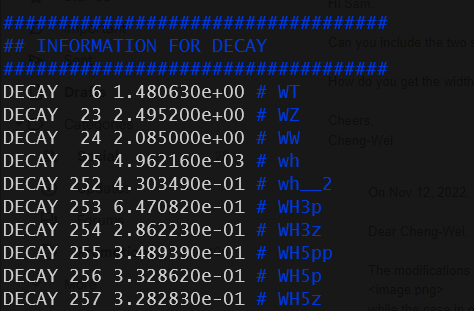
\includegraphics[width=0.4\textwidth]{decay_width.png}
		}
		\subfloat[Modified]{
			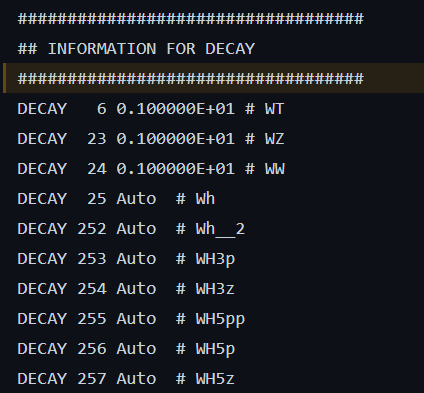
\includegraphics[width=0.4\textwidth]{decay_width_modified.png}
		}
		\caption{Left is the original decay widths in MadGraph. The right is the decay widths in Janice's parameter card.}
		\label{fig:decay_width}
	\end{figure}

	
	\subsection{Sample selection}% (fold)
	\label{sub:sample_selection}
		Sample selection criteria:
		\begin{enumerate}
			\item The transverse momentum of jets are required $p_\text{T} \in (350, 450) \text{GeV}$ and in range $\abs{\eta}<1$.
			\item Merging: The angular distance between the two quarks decayed from the vector boson is required $\Delta R(q_1,q_2) < 0.6$.
			\item Matching: The vector boson and jet are matched if $\Delta R(V,j) < 0.1$. 
		\end{enumerate}

		The training samples are constructed from the vector bosons that pass these criteria. All the vector bosons passing the criteria are included, even for the events with only one vector boson passing the criteria.

	% subsection sample_selection (end)
	\subsection{Jet image}% (fold)
	\label{sub:jet_image}
		After the sample selection, we can construct the jet image of the matching vector boson jets. The jet image is constructed after preprocessing procedure, including centralization, rotation, flipping, and pixelating.

		For some events, the vector boson jet will cross the $\phi = \pm\pi$ boundary, which will make the centralization step fail. We will plus the $\phi$ coordinate of jet constituents by $\pi$ so that its center is around $\phi=0$. This has also have done in Janice's code.

	% subsection jet_image (end)	
	\subsection{Plots}% (fold)
	\label{sub:plots}
		For the following figures, the sample sizes are $(W^{+}, W^{-},Z) = (\text{350 k}, \text{364 k}, \text{316 k})$.

		Figure \ref{fig:jet_mass_distribution} demonstrates the jet mass distribution.
		\begin{figure}[htpb]
			\centering
			\subfloat[Paper]{
			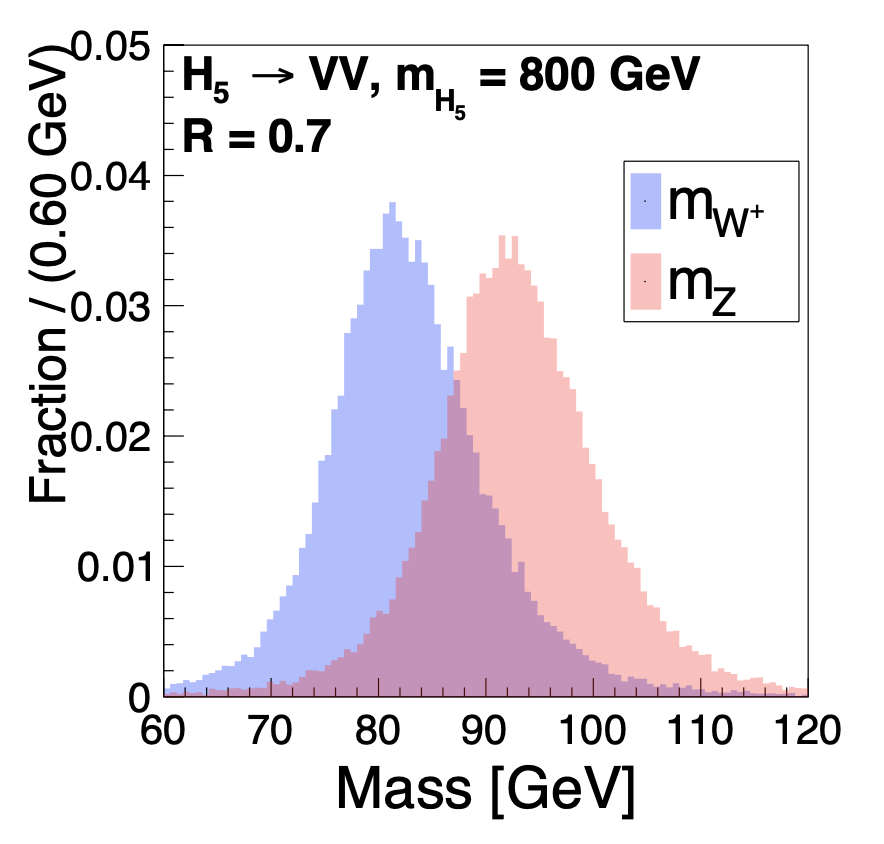
\includegraphics[width=0.48\textwidth]{jet_mass_distribution_paper.png}
			}
			\subfloat[Ours]{
				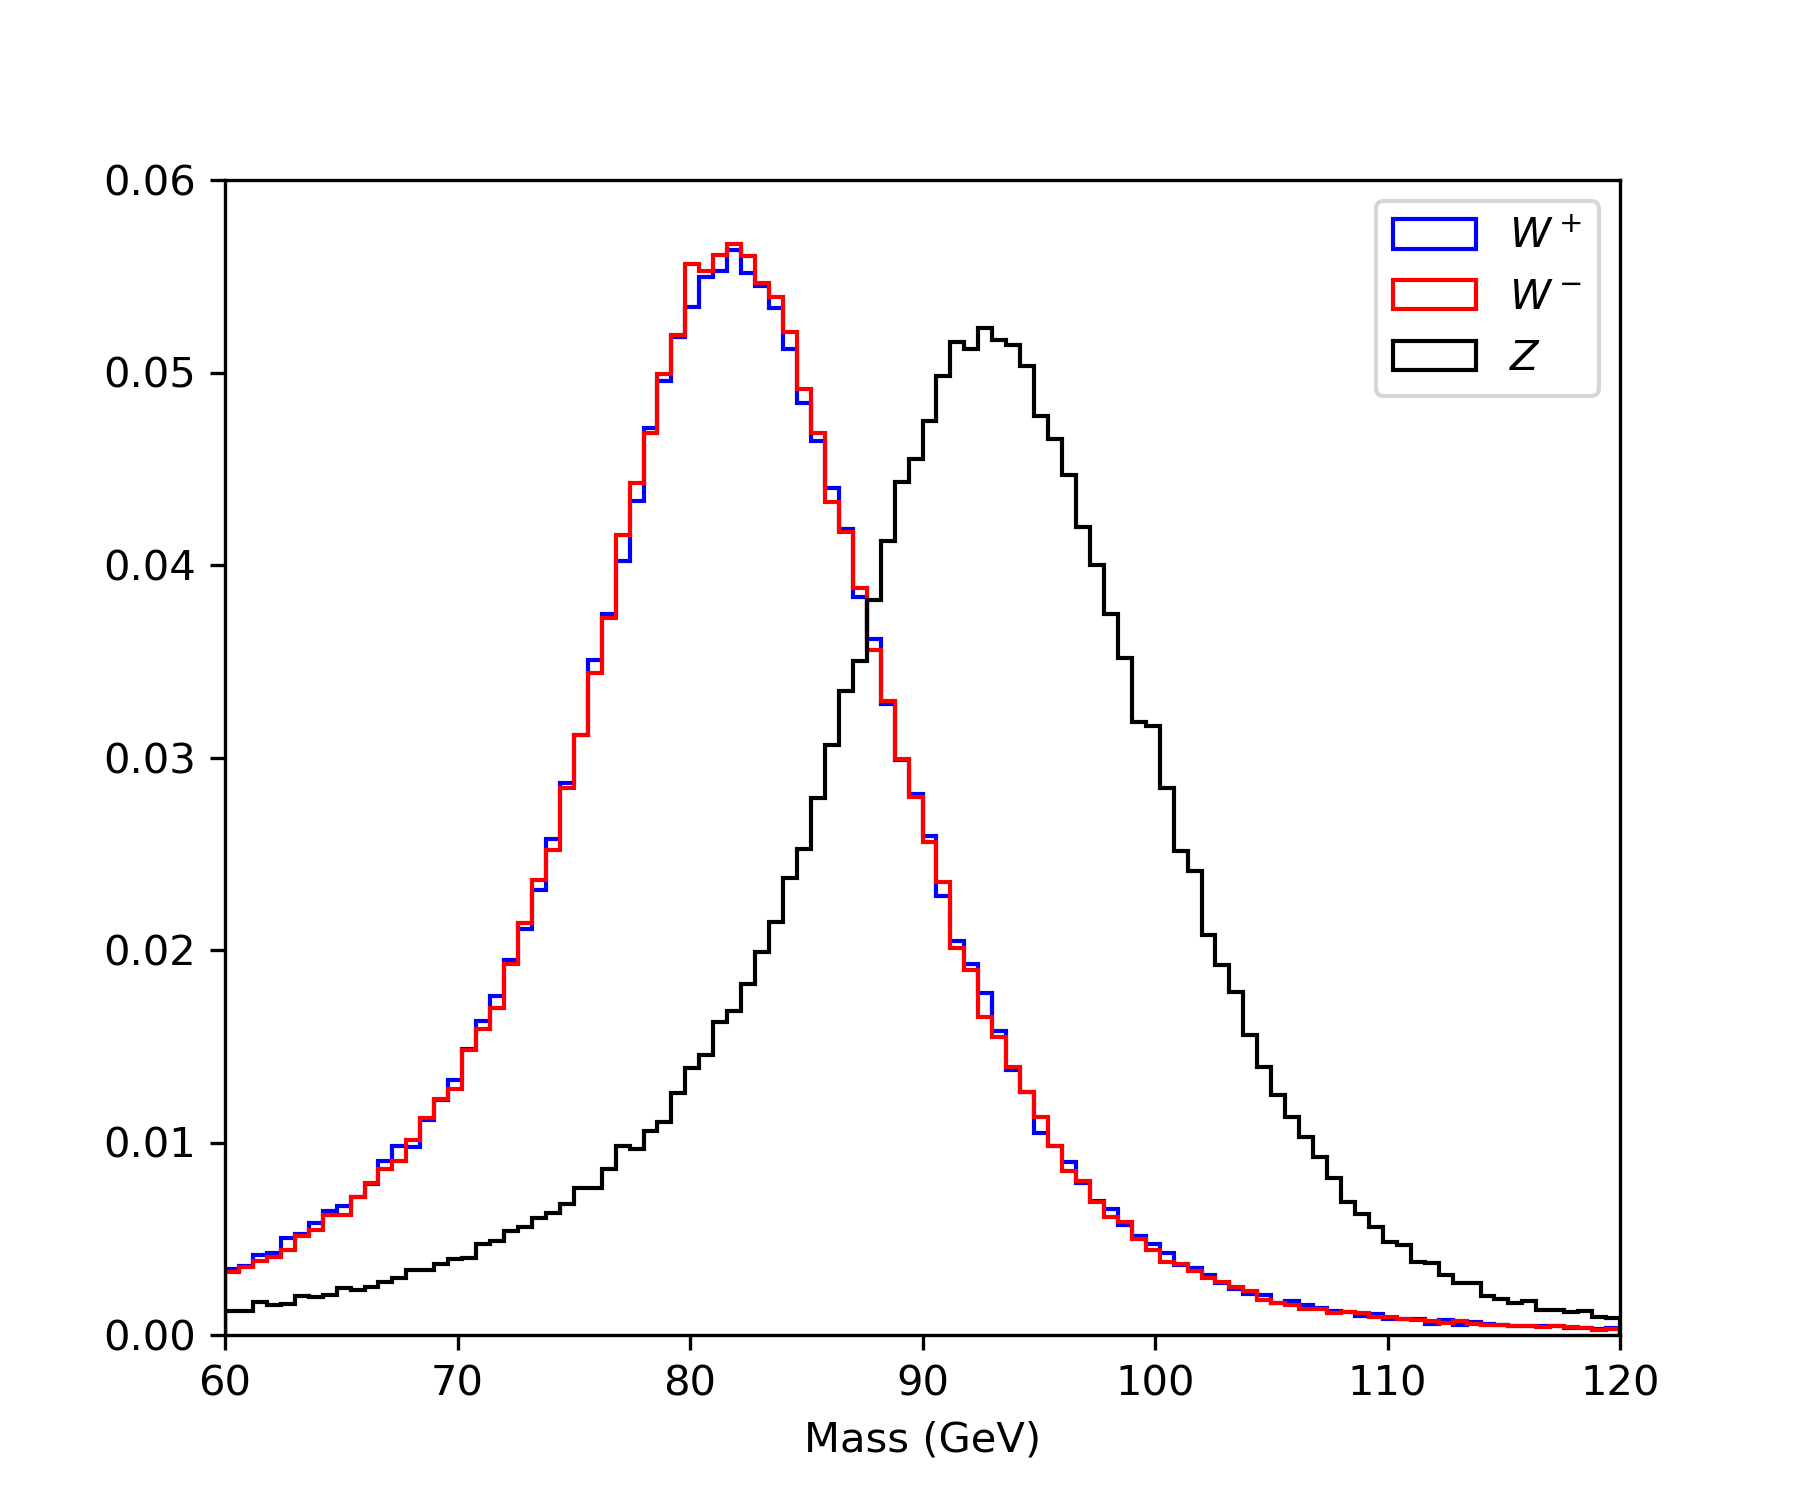
\includegraphics[width=0.48\textwidth]{jet_mass_distribution.png}
			}
			\caption{Jet mass distribution of their vector boson samples.}
			\label{fig:jet_mass_distribution}
		\end{figure}

		Figure \ref{fig:jet_charge_different_kappa} shows the jet charge distributions with different $\kappa$.
		\begin{figure}[htpb]
			\centering
			\subfloat[Paper]{
				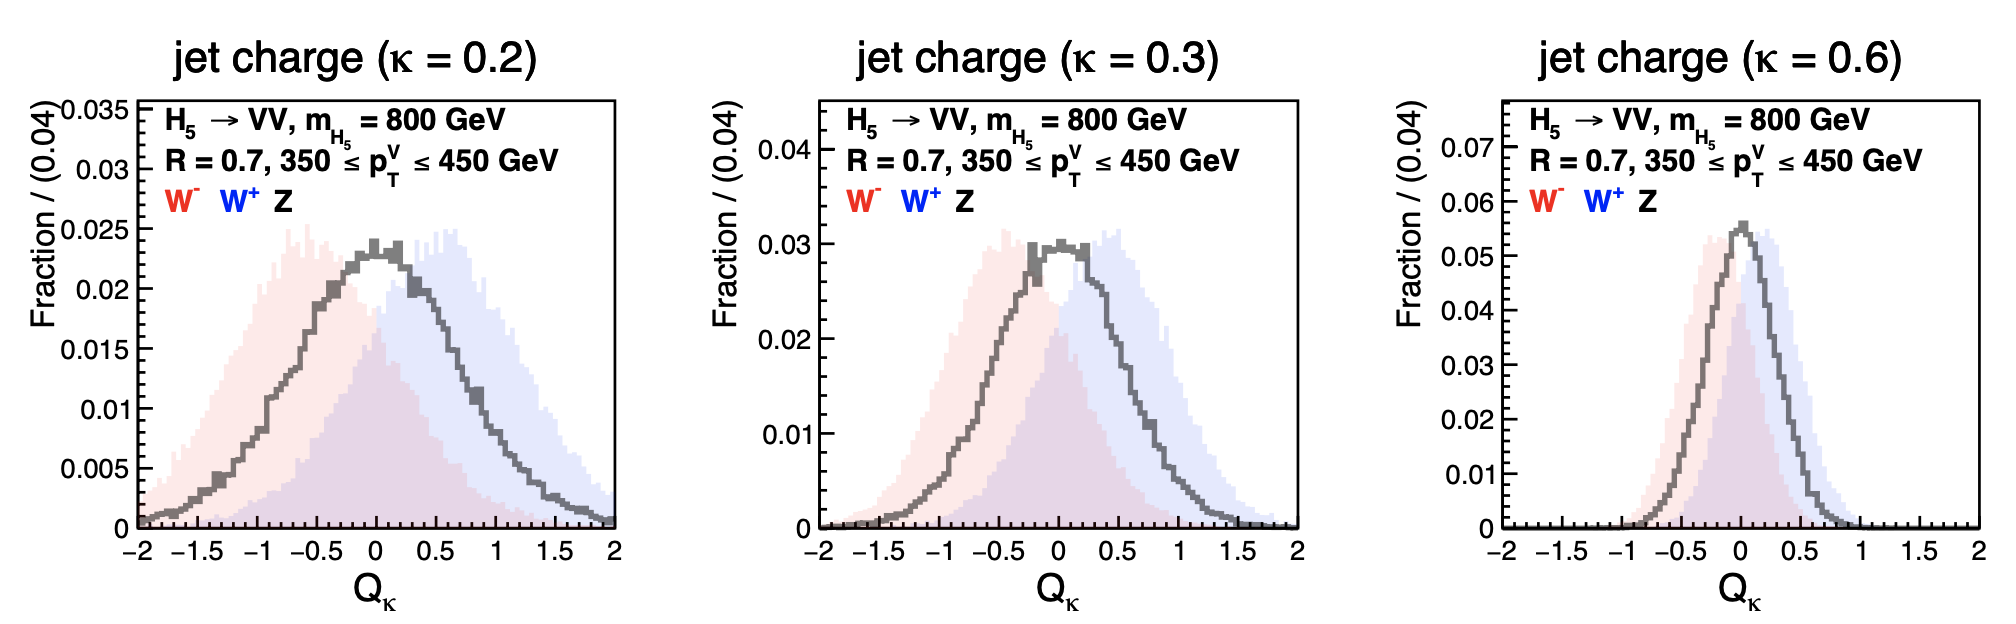
\includegraphics[width=0.95\textwidth]{jet_charge_distribution_paper.png}
			} 
			\\
			\subfloat[Ours]{
				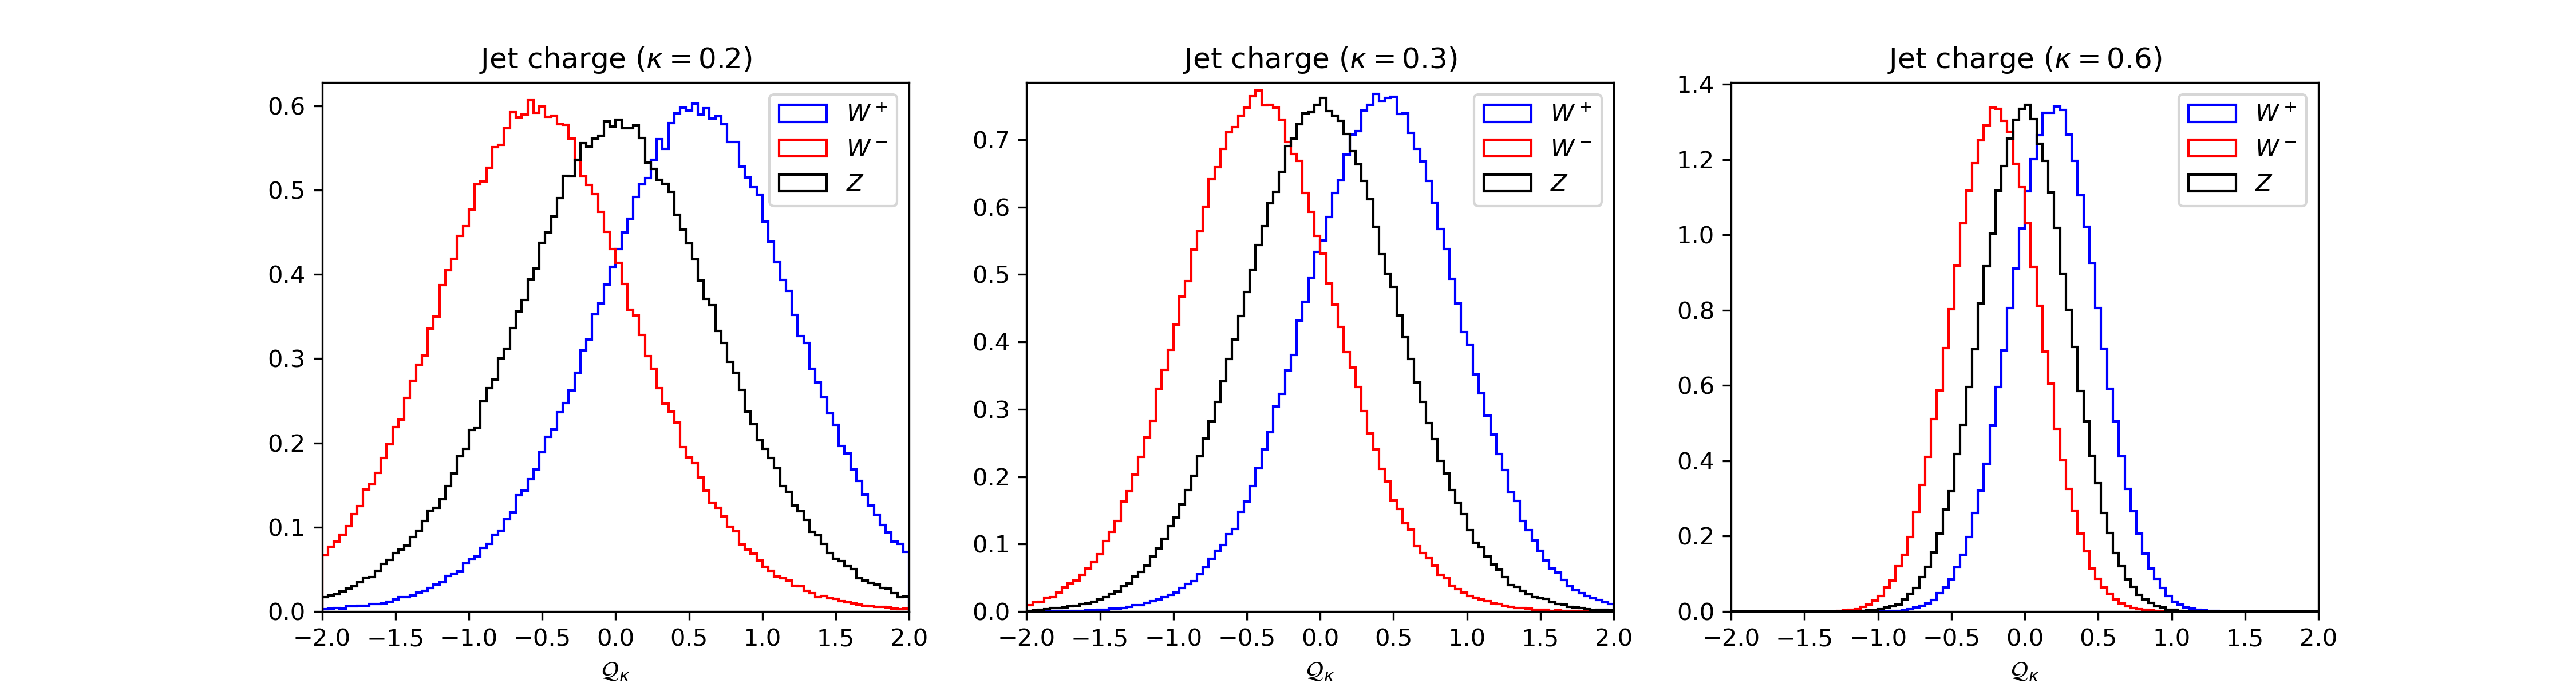
\includegraphics[width=1.00\textwidth]{jet_charge_distribution.png}
			}
			\caption{$\mathcal{Q}_\kappa$ distribution of vector boson samples.}
			\label{fig:jet_charge_different_kappa}
		\end{figure}

		Figure \ref{fig:jet_image_PT}, \ref{fig:jet_image_Qk} shows the average jet images of $p_\text{T}$ and $\mathcal{Q}_\kappa$.
		\begin{figure}[htpb]
			\centering
			\subfloat[Paper]{
				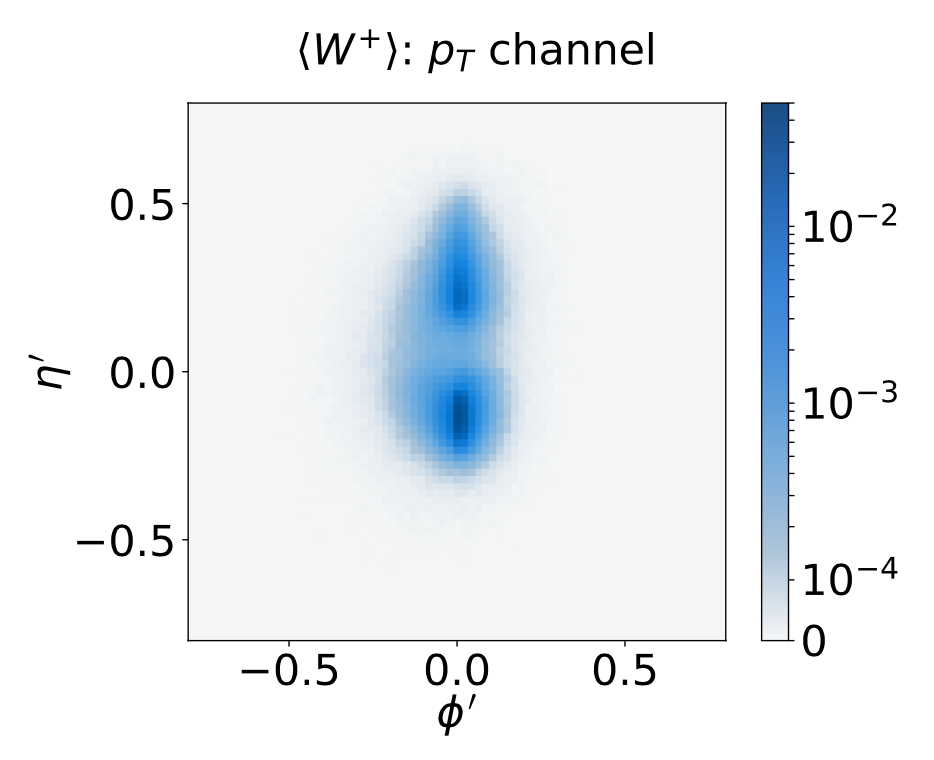
\includegraphics[width=0.50\textwidth]{jet_image_PT_paper.png}
			} 
			\\
			\subfloat[Ours]{
				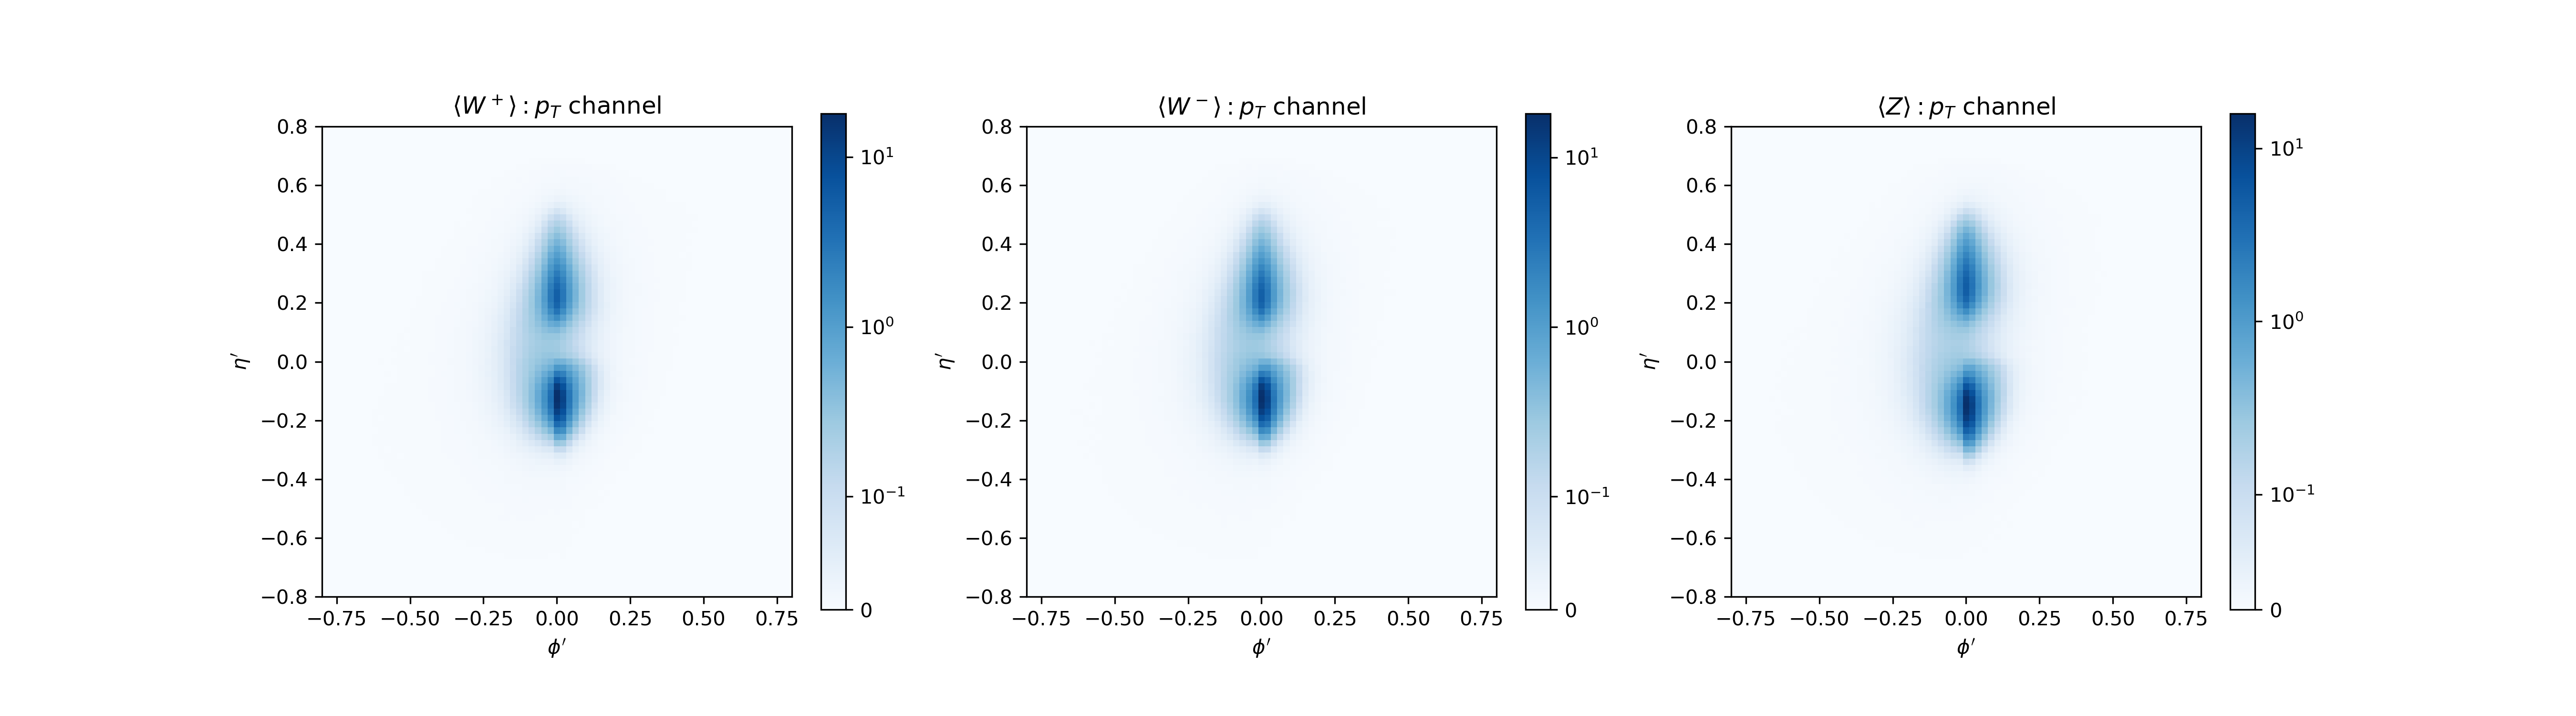
\includegraphics[width=0.95\textwidth]{jet_image_PT.png}
			}
			\caption{Average of jet images in the $p_\text{T}$ channel.}
			\label{fig:jet_image_PT}
		\end{figure}
		\begin{figure}[htpb]
			\centering
			\subfloat[Paper]{
				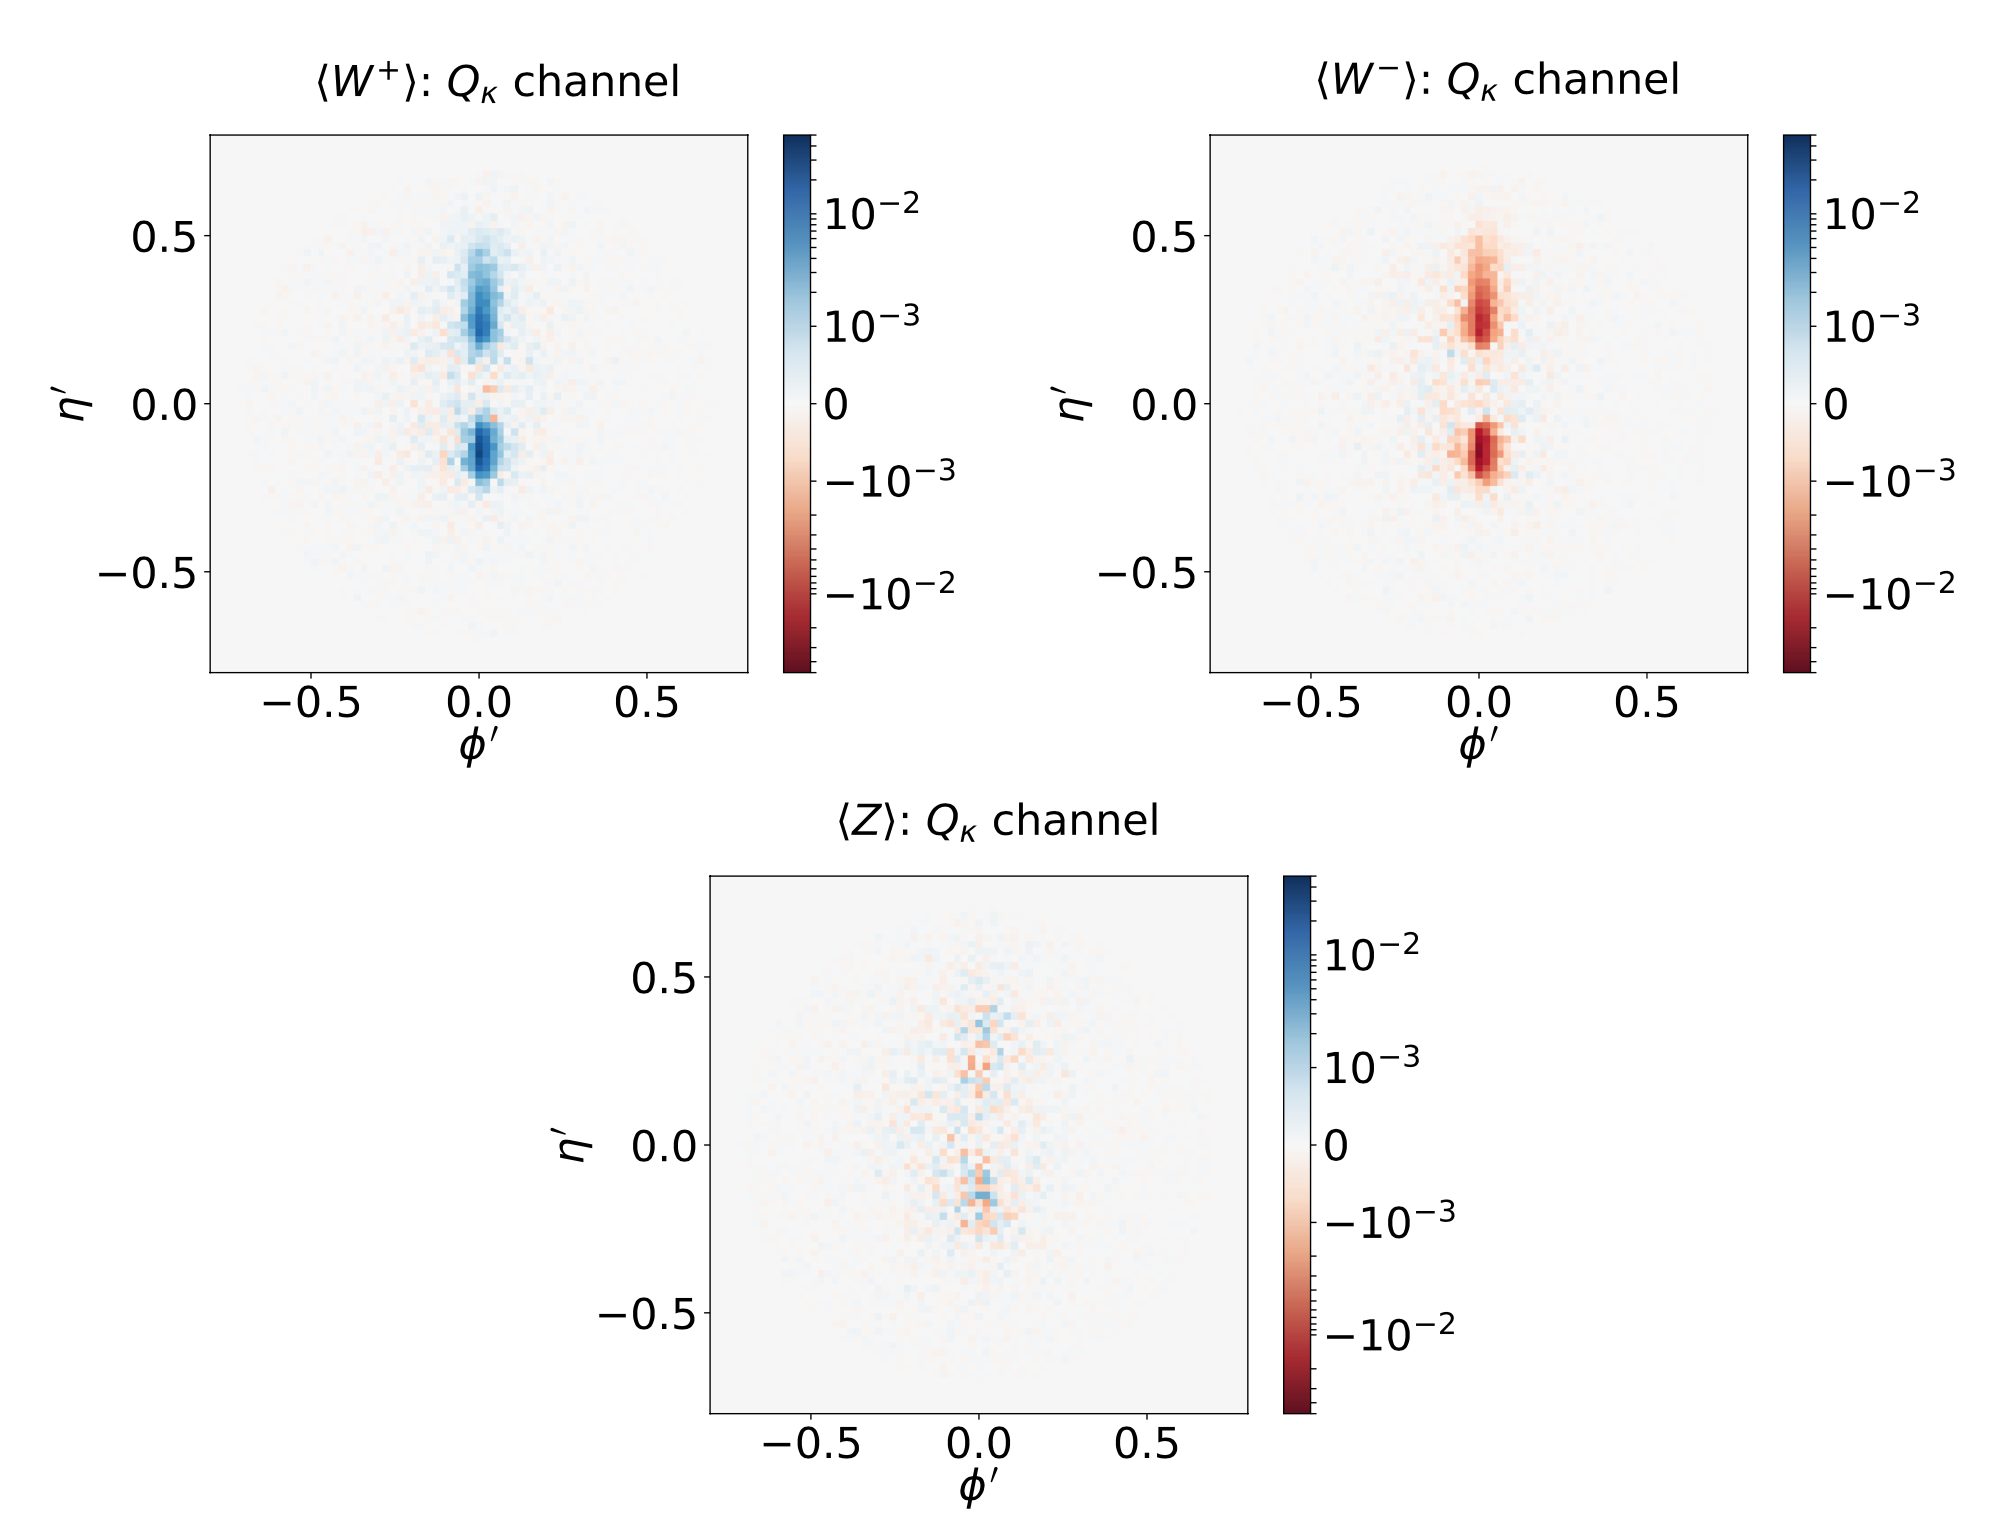
\includegraphics[width=0.95\textwidth]{jet_image_Qk_paper.png}
			} 
			\\
			\subfloat[Ours]{
				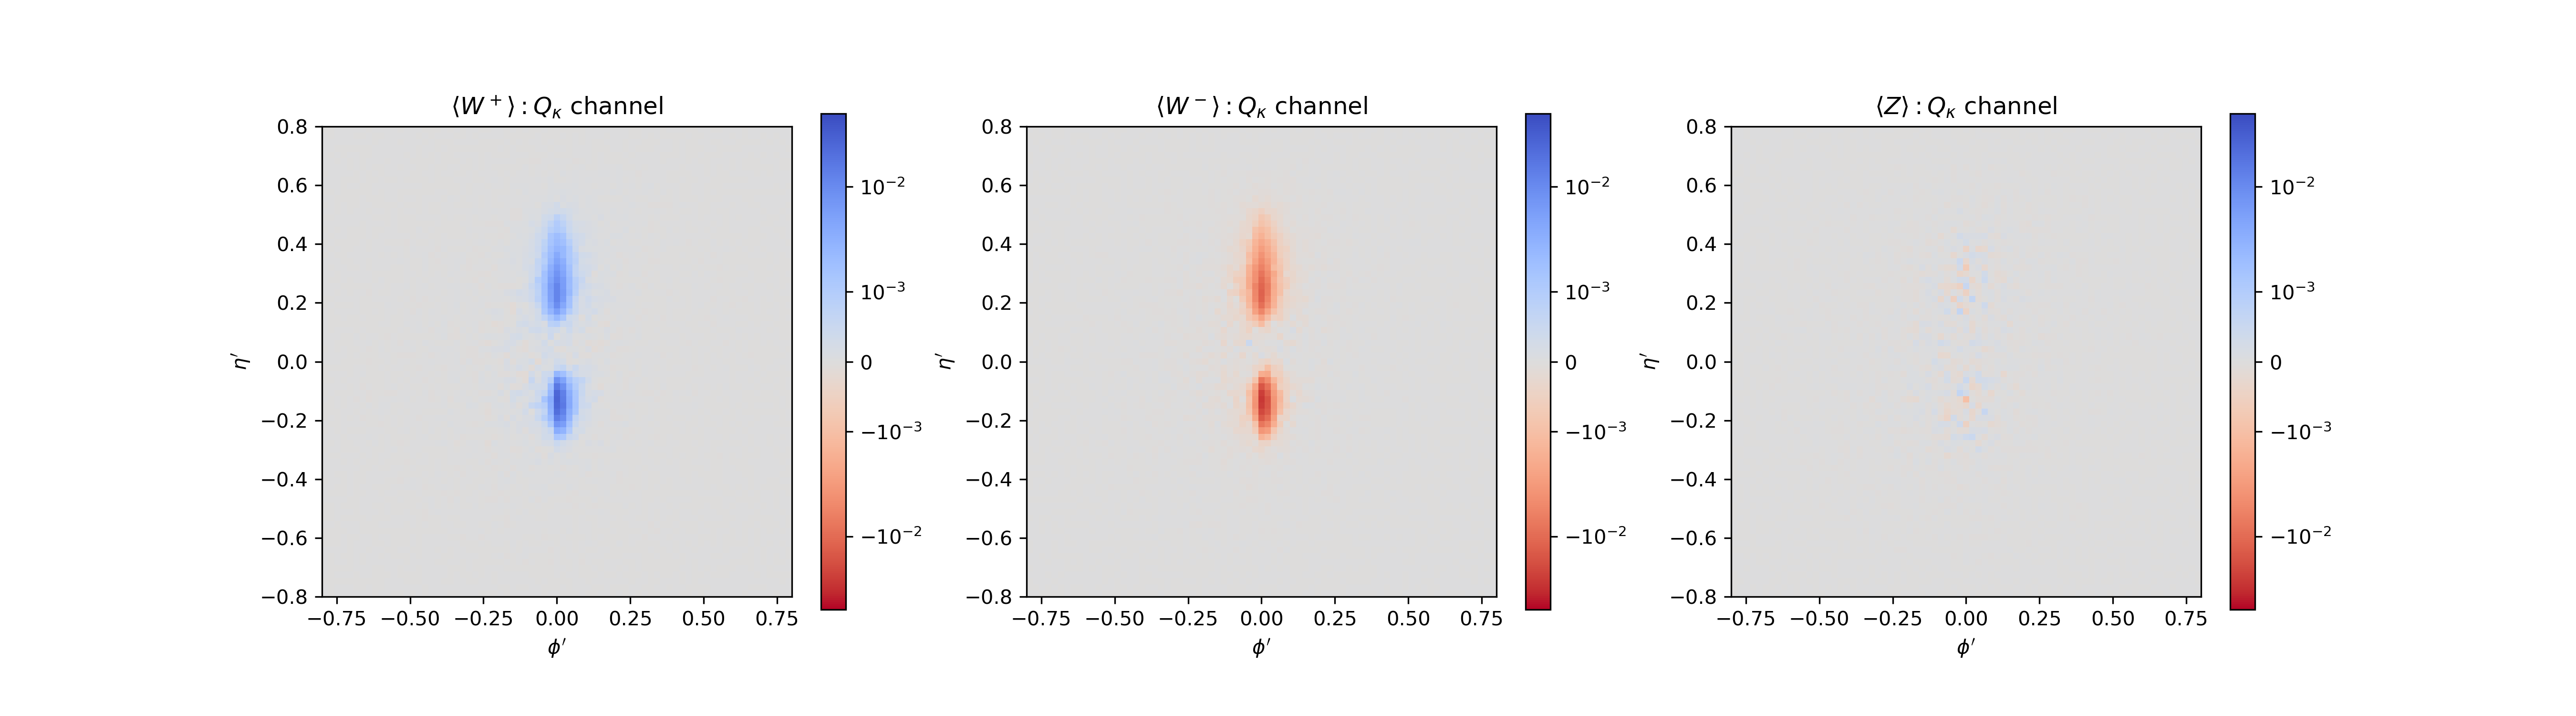
\includegraphics[width=0.95\textwidth]{jet_image_Qk.png}
			}
			\caption{Average of jet images in the $\mathcal{Q}_\kappa$ channel, with $\kappa = 0.15$.}
			\label{fig:jet_image_Qk}
		\end{figure}

		Figure \ref{fig:jet_image_PT_Z-W+} presents the $Z$ jet image minus $W^{+}$ jet image in $p_\text{T}$ channel.
		\begin{figure}[htpb]
			\centering
			\subfloat[Paper]{
				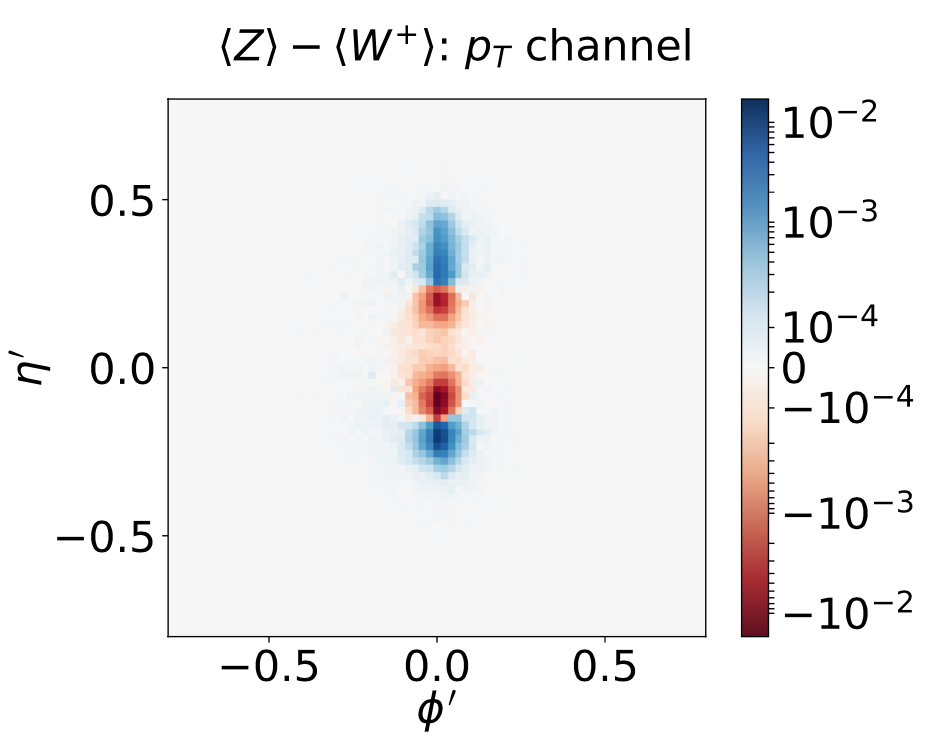
\includegraphics[width=0.5\textwidth]{jet_image_PT_Z-W+_paper.png}
			}
			\subfloat[Ours]{
				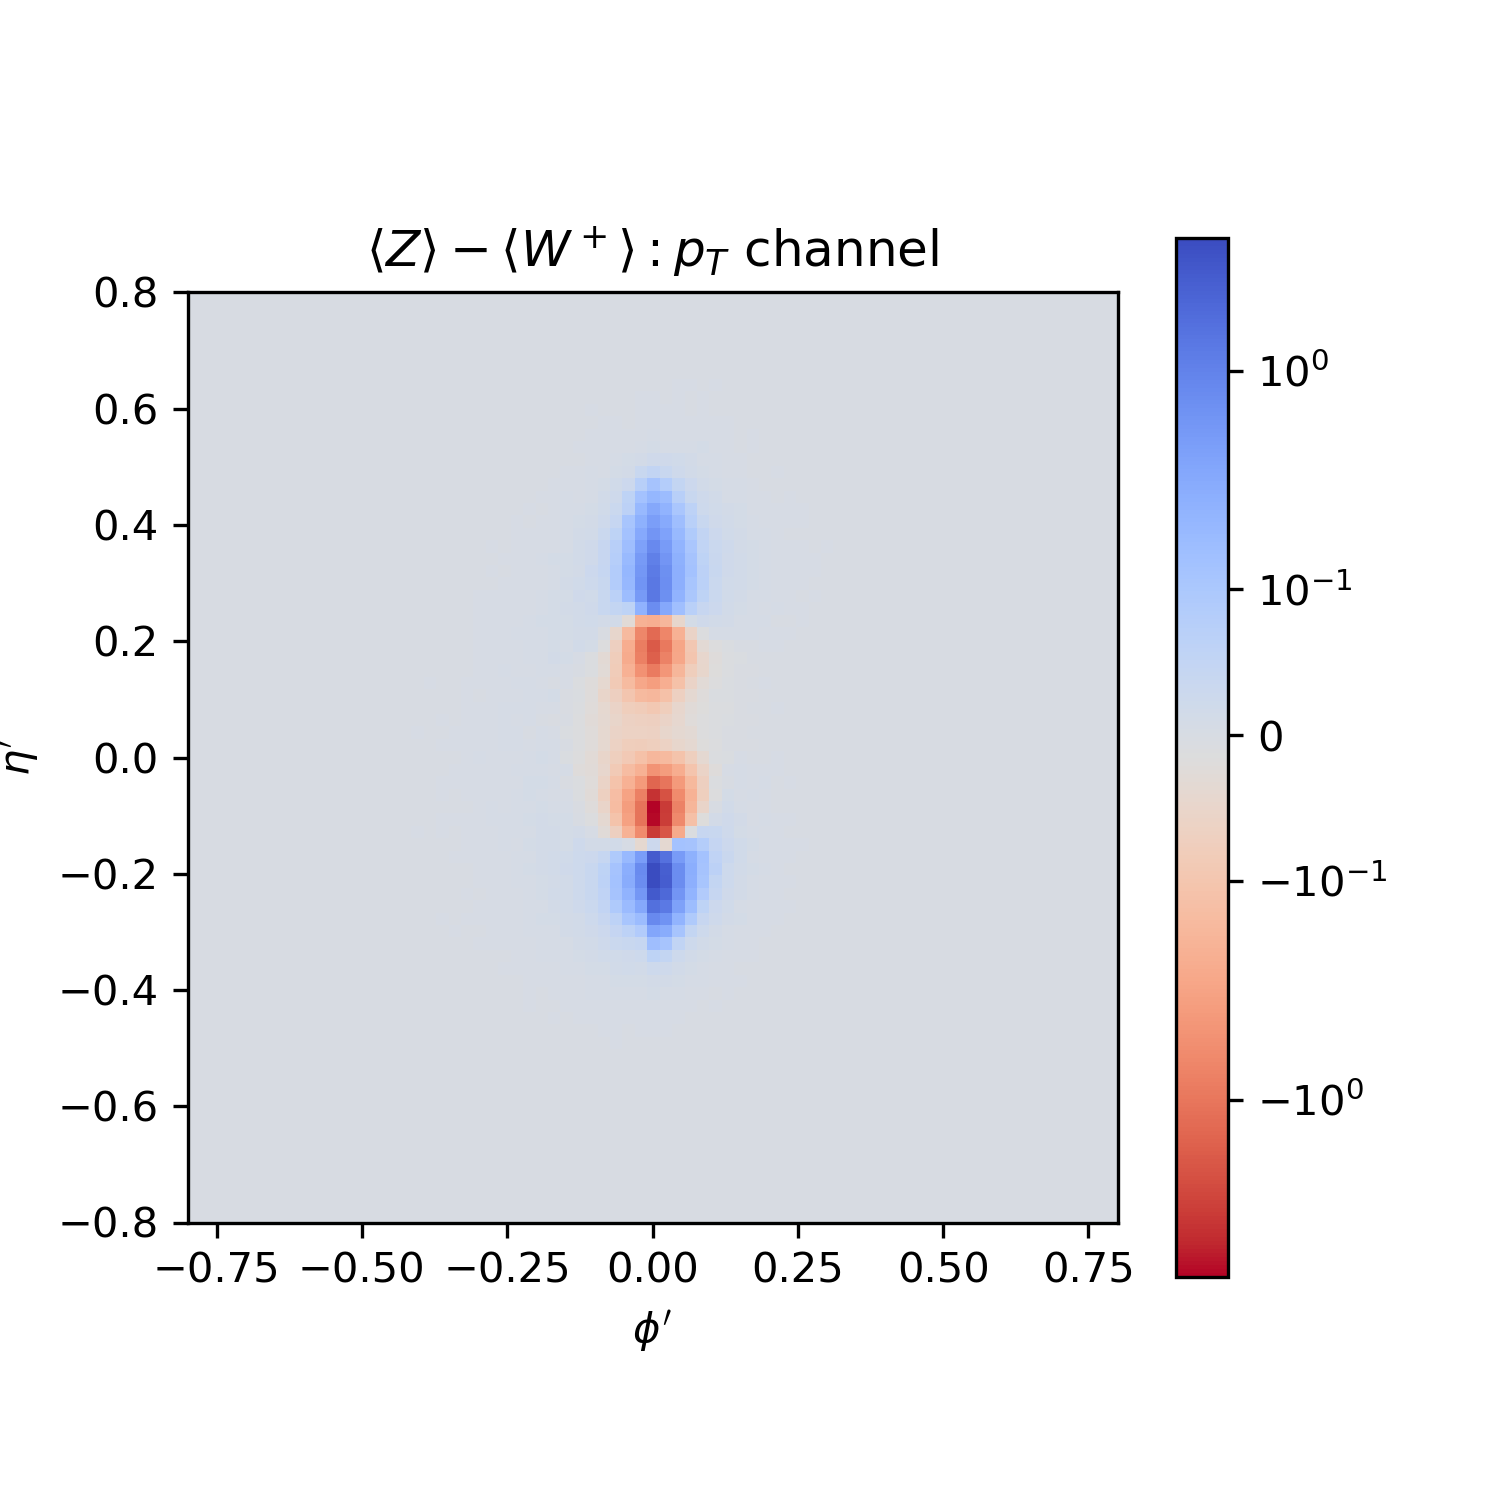
\includegraphics[width=0.5\textwidth]{jet_image_PT_Z-W+.png}
			}
			\caption{The difference between the $Z$ and $W^{+}$ average jet images in $p_\text{T}$ channel.}
			\label{fig:jet_image_PT_Z-W+}
		\end{figure}

	% subsection plots (end)	
% section preparation_of_sample (end)
\section{Ternary classification}% (fold)
\label{sec:ternary_classification}
		The training, validation, and testing sample sizes are shown in Table \ref{tab:sample_size}. The BDT training features are jet mass and jet charge. The CNN training features are the jet image with $p_\text{T}$ and $\mathcal{Q}_\kappa$.
		\begin{table}[htpb]
			\centering
			\caption{The entries in the sum correspond to the $(W^{+}, W^{-}, Z)$ samples.}
			\label{tab:sample_size}
			\begin{tabular}{c|c|c|c}
			Case & Training set     & Validation set & Testing set   \\ \hline
			Paper& $169k+178k+157k$ & $19k+20k+18k$  & $60k+64k+55k$ \\
			1    & $224k+232k+201k$ & $56k+58k+50k$  & $69k+72k+63k$ \\
			\end{tabular}
		\end{table}

		The training results are summarized in Table \ref{tab:training_result}.
		\begin{table}[htpb]
			\centering
			\caption{The training results of Janice's paper and ours. The AUC and ACC values of the testing results, expressed in percentage, for BDT, CNN, and CNN$^2$ models. The CNN and CNN$^2$ models are presented with an average performance and a standard deviation value since they are trained over ten times with the same training data set. Yet, the value in the parenthesis for the ACC value of each boson is only derived from a single result.}
			\label{tab:training_result}
			\resizebox{\textwidth}{!}{
			\begin{tabular}{c|c|c|cc|cc|cc}
										&					  &             & \multicolumn{2}{c|}{$W^{+}$} & \multicolumn{2}{c|}{$W^{-}$} & \multicolumn{2}{c}{$Z$} \\
										& Sample			  & Overall ACC & AUC        & ACC       & AUC        & ACC       & AUC       & ACC       \\ \hline
				BDT $\kappa=0.30$       &\multirow{3}{*}{Paper}& 66.8 & N.A.  & N.A.  & 83.5 & 75.8 & 83.7 & 77.3\\
				CNN $\kappa=0.15$       &					   & 72.0 & N.A.  & N.A.  & 87.2 & 78.9 & 89.4 & 81.7\\
				CNN${}^2$ $\kappa=0.15$ &					   & 73.2 & N.A.  & N.A.  & 87.6 & 79.5 & 90.9 & 83.3\\ \hline
				BDT $\kappa=0.30$       &\multirow{3}{*}{1}    & 65.9 & 82.9 & 77.7 & 82.9 & 77.5 & 80.9 & 78.4\\
				CNN $\kappa=0.15$       &					   & 69.76$\pm$0.06 & 86.46$\pm$0.02 & (80.4) & 86.34$\pm$0.02 & (79.6) & 83.80$\pm$0.04 & (81.2)\\
				CNN$^2$ $\kappa=0.15$   &					   & 69.80$\pm$0.05 & 86.30$\pm$0.02 & (80.0) & 86.19$\pm$0.02 & (79.7) & 84.39$\pm$0.05 & (81.8)\\
			\end{tabular}
			}
		\end{table}	

		By doing the CNN and CNN$^2$ training many times, we found that the phase transition stated in Janice's paper seldom shows up. For most training processes, the accuracy ends up with $65\%$ in the first epoch and smoothly increases to the highest value. The loss and learning curve of CNN and CNN$^2$ models are illustrated in Figure \ref{fig:CNN learning curve}. We also show the ROC curve in Figure \ref{fig:CNN roc curve}
		\begin{figure}[htpb]
			\centering
			\subfloat[Ours]{
				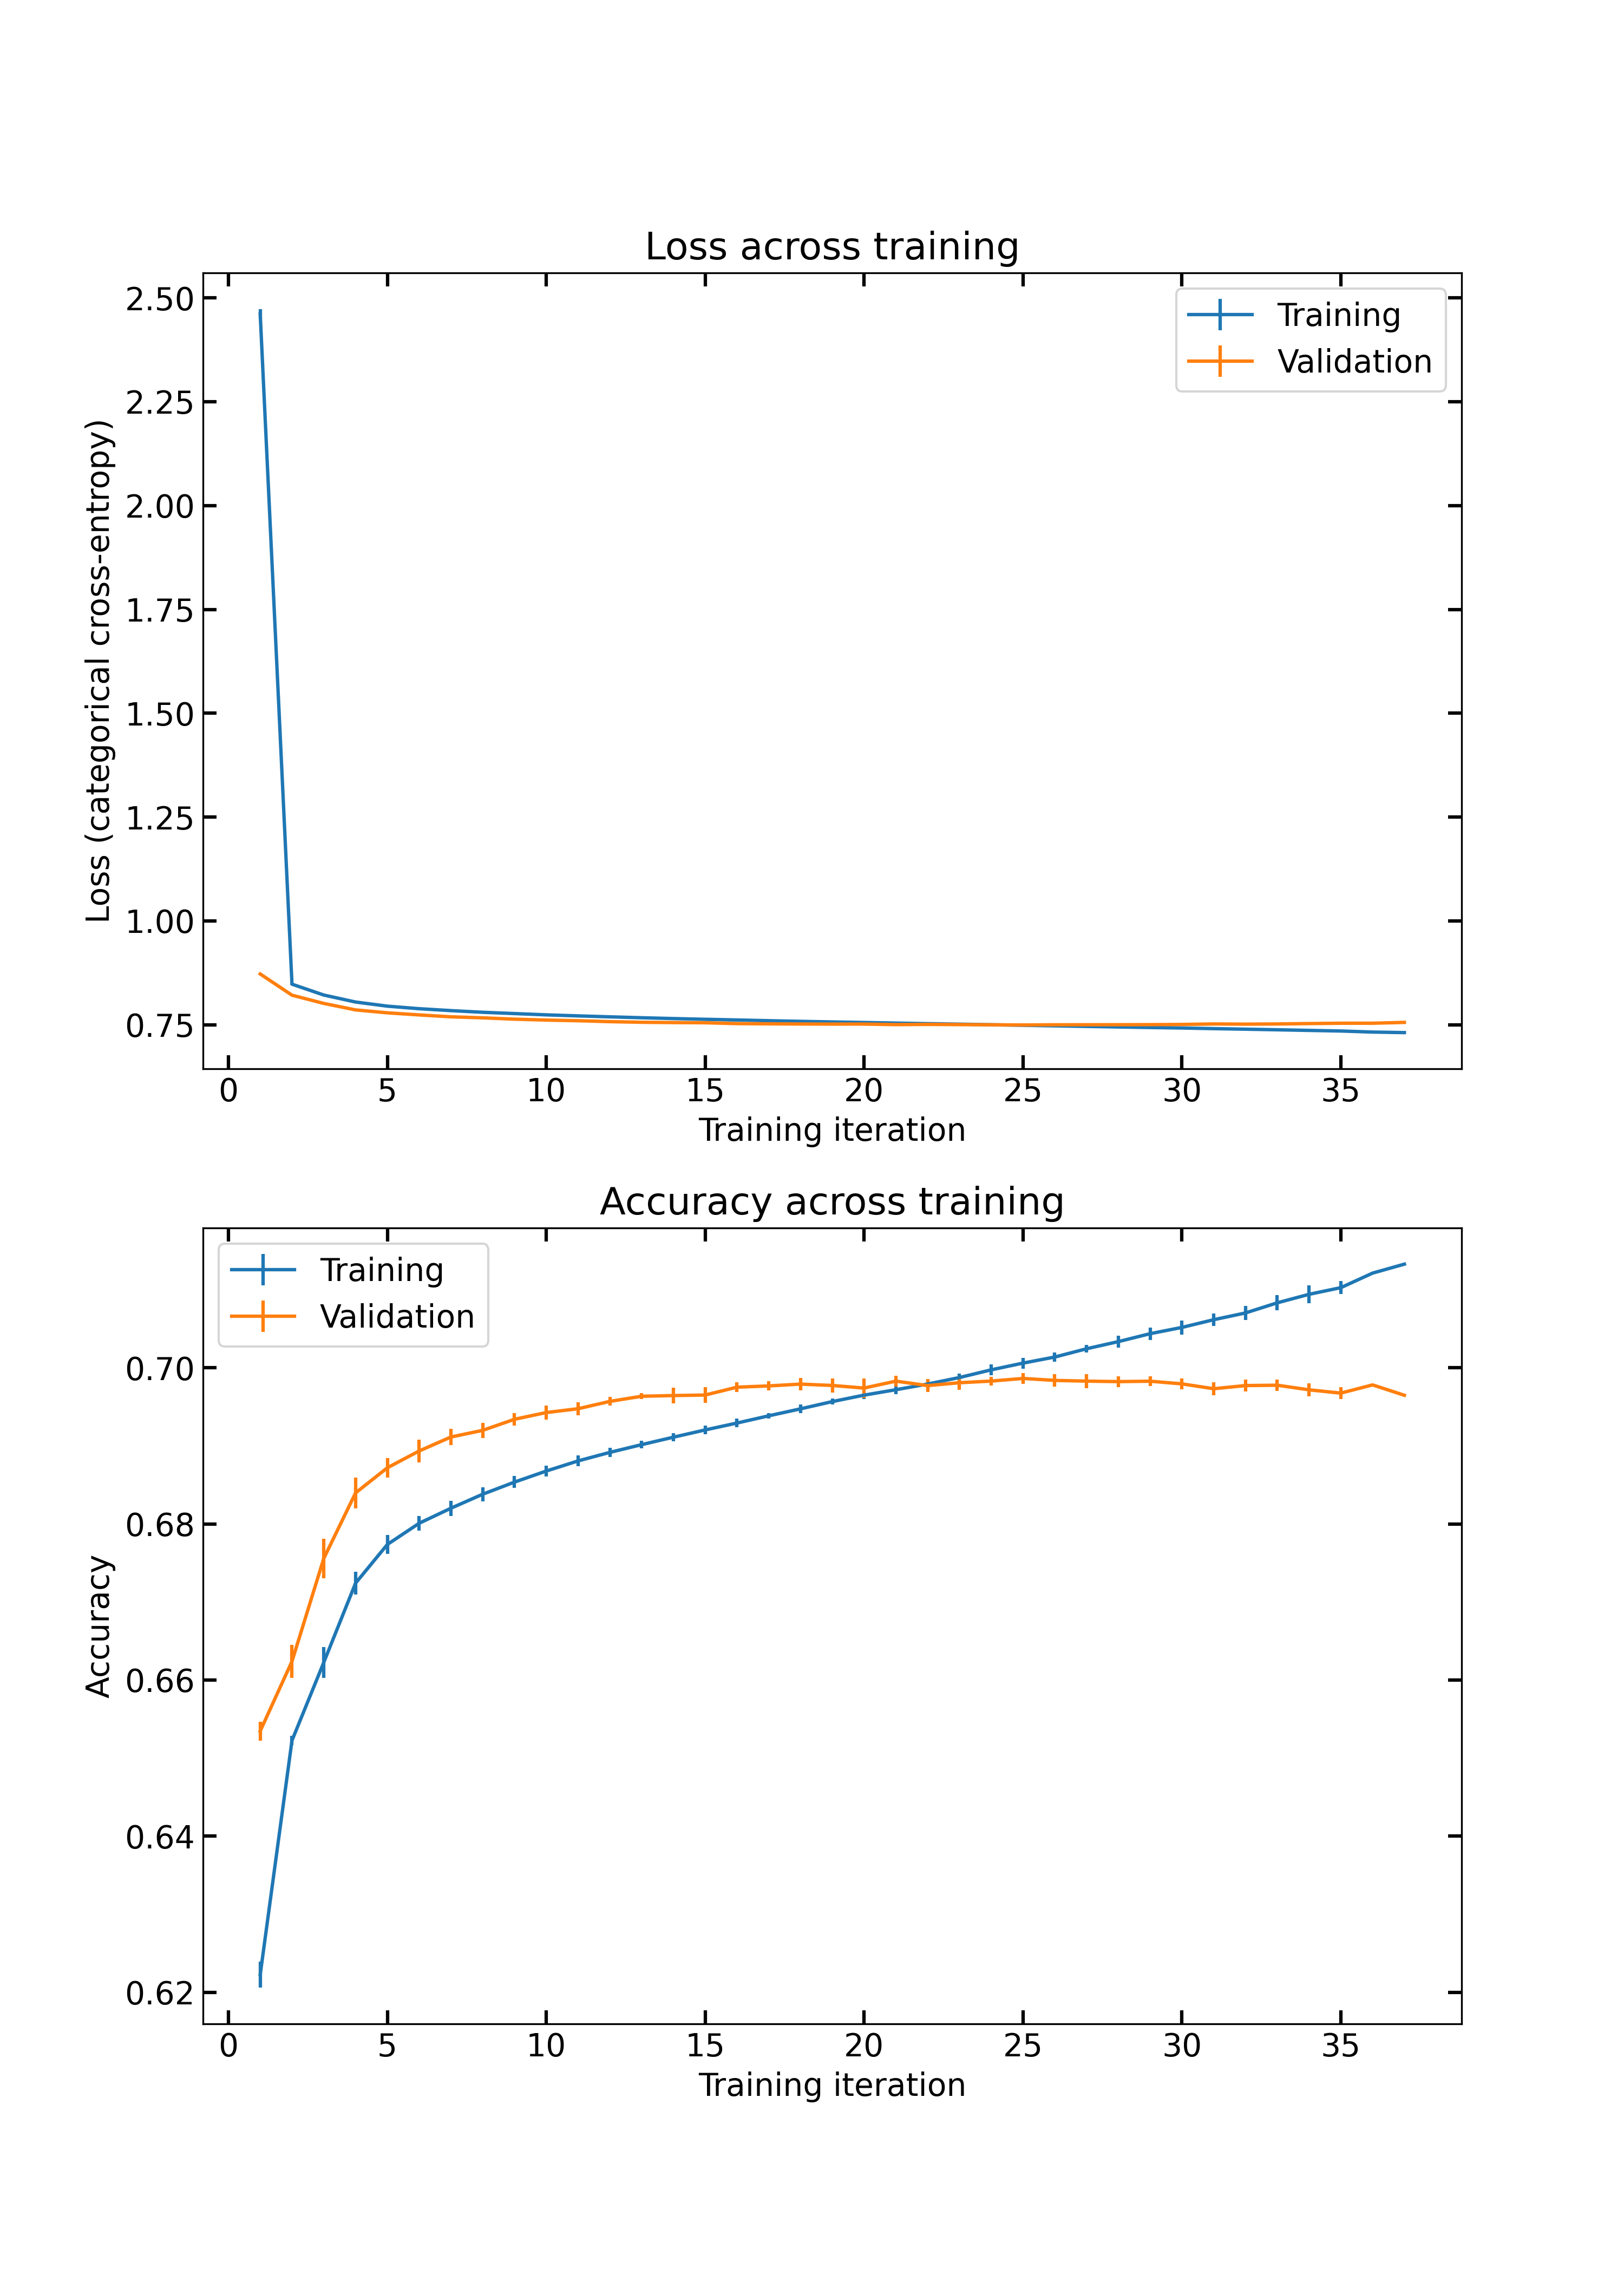
\includegraphics[width=0.95\textwidth]{loss and accuracy_CNN.png}
			} 
			\caption{The loss and learning curve for the CNN model. Both of them are demonstrated with the average value (solid curve) and the first standard deviation range (error bar).}
			\label{fig:CNN learning curve}
		\end{figure}
		\begin{figure}[htpb]
			\centering
			\subfloat[Ours]{
				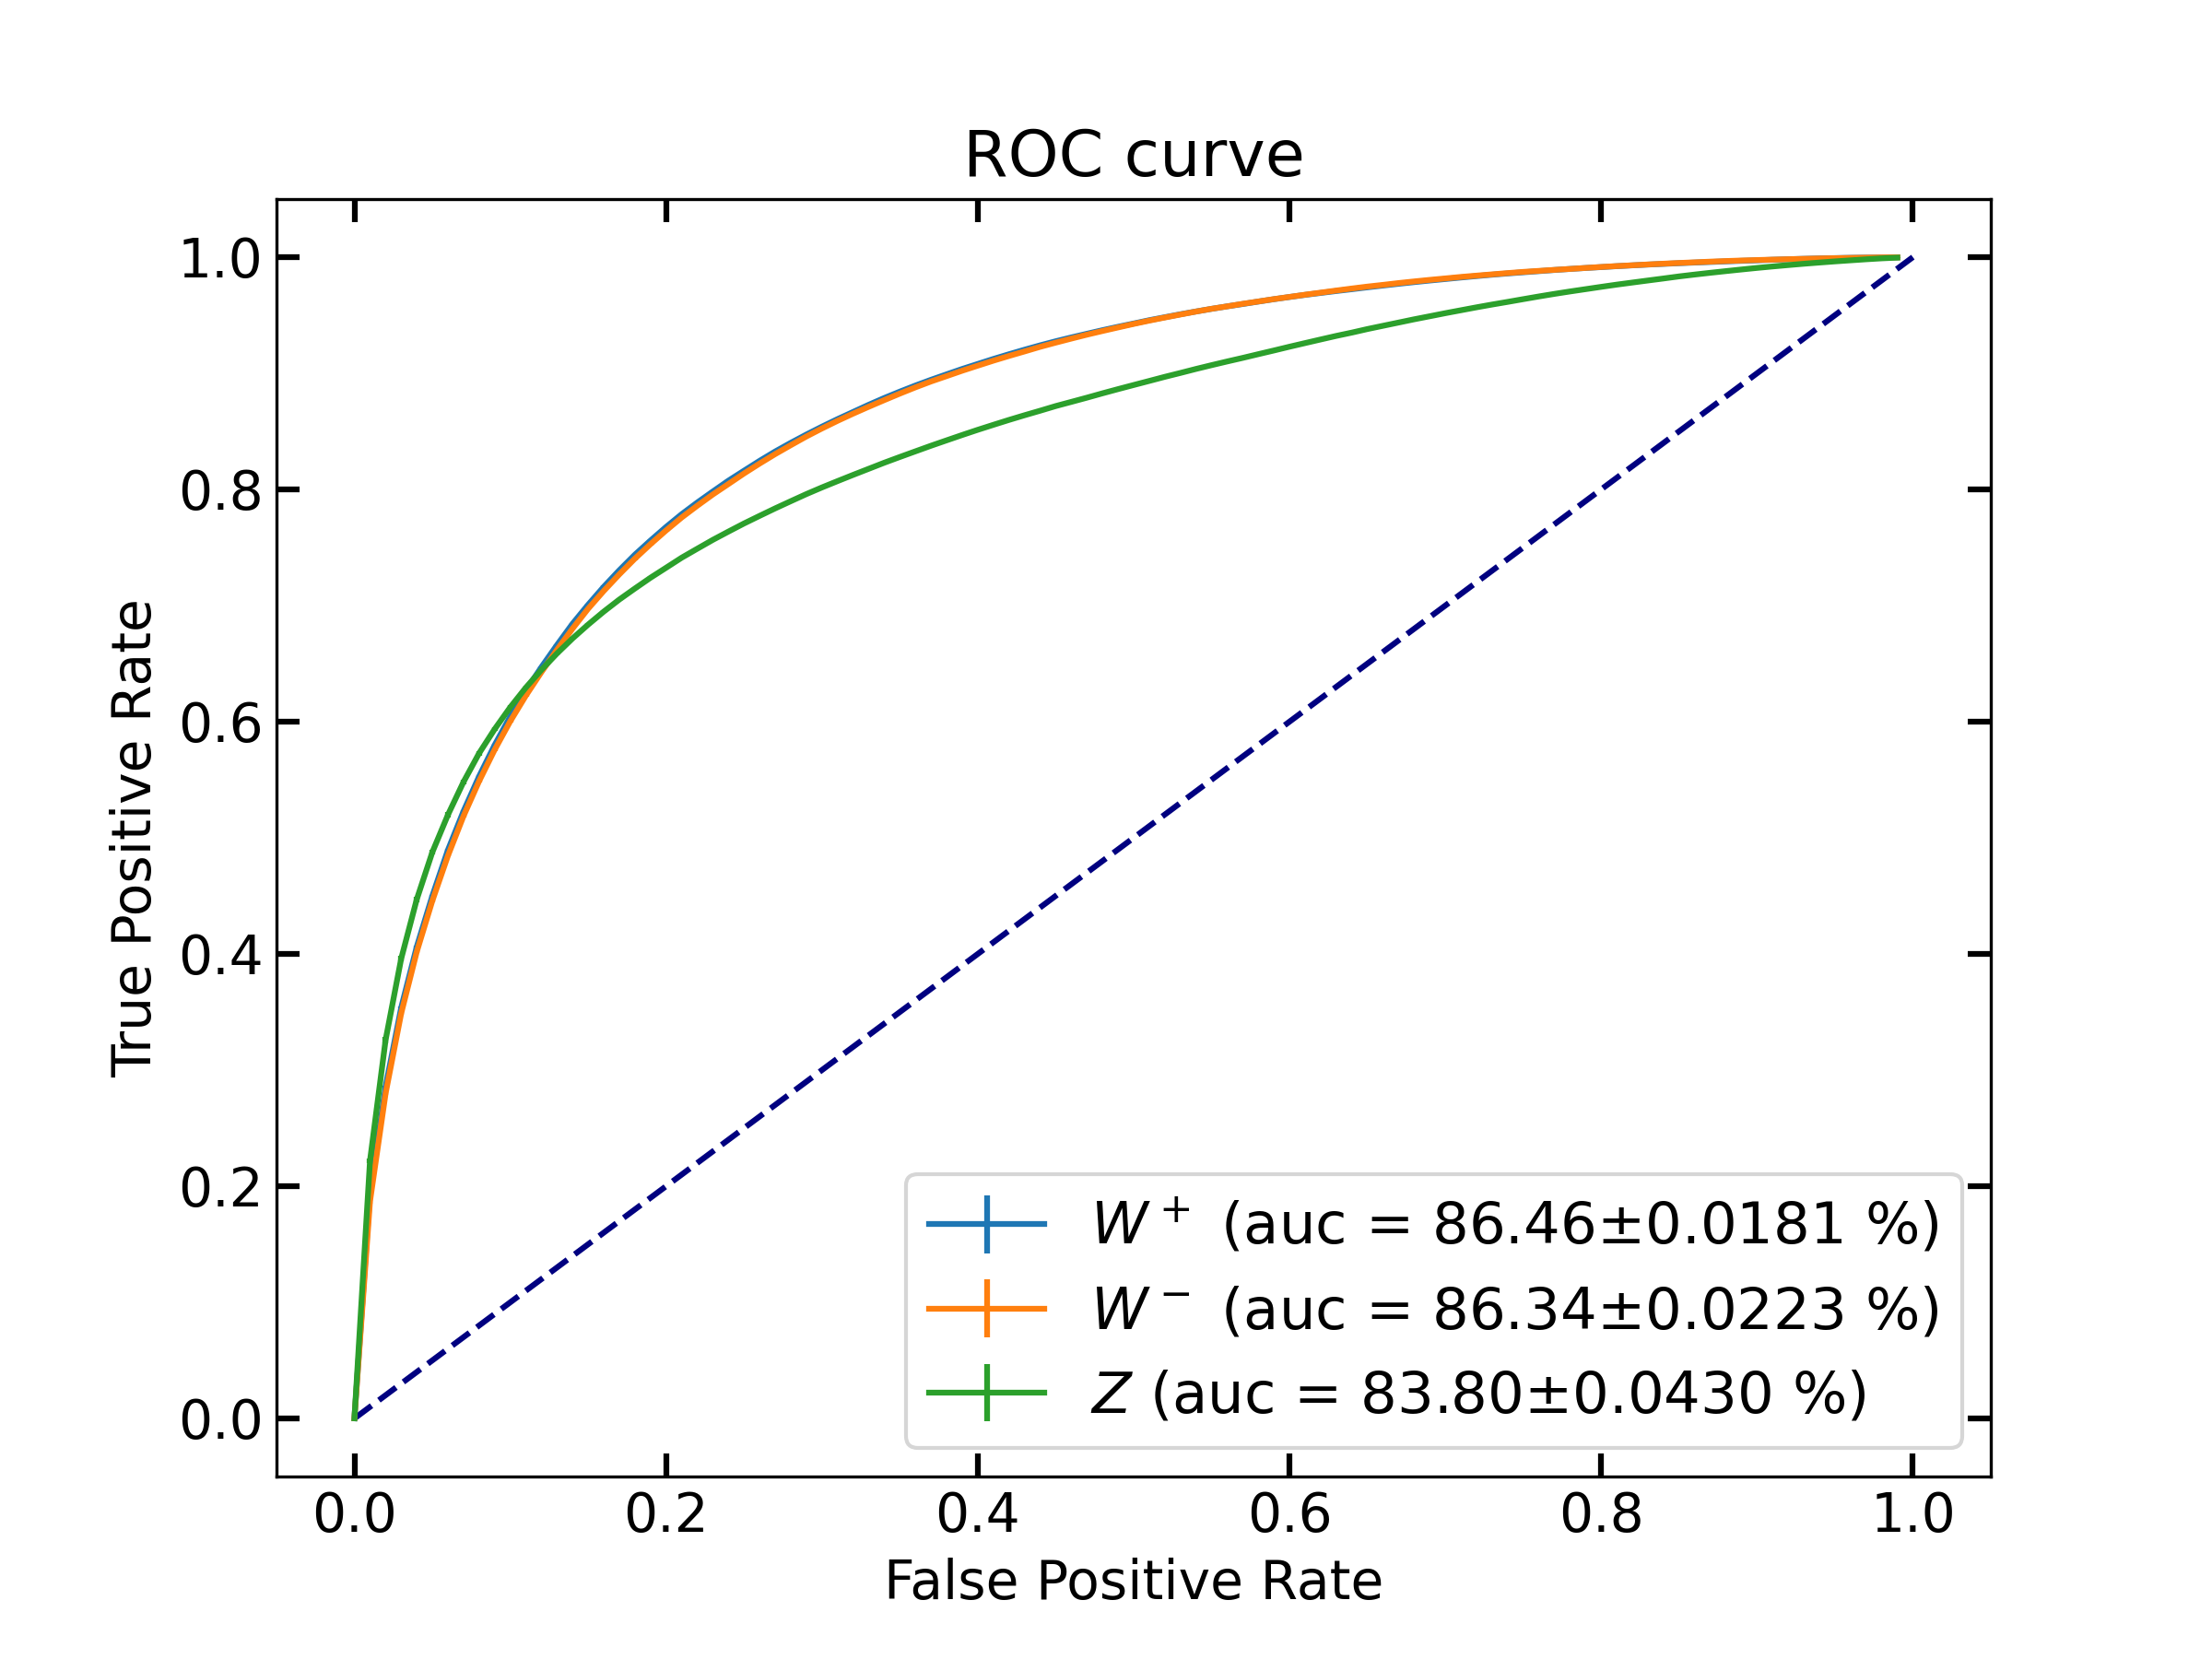
\includegraphics[width=0.95\textwidth]{roc_auc_CNN.png}
			} 
			\caption{The ROC curve of each vector boson for the CNN model. The plotting scheme is the same as Figure~\ref{fig:CNN learning curve}.}
			\label{fig:CNN roc curve}
		\end{figure}
		
		Here we provide the loss and learning curve and the ROC curve for the CNN$^2$ model in Figure~\ref{fig:CNNsq learning curve} and Figure~\ref{fig:CNNsq roc curve}.
		\begin{figure}[htpb]
			\centering
			\subfloat[Ours]{
				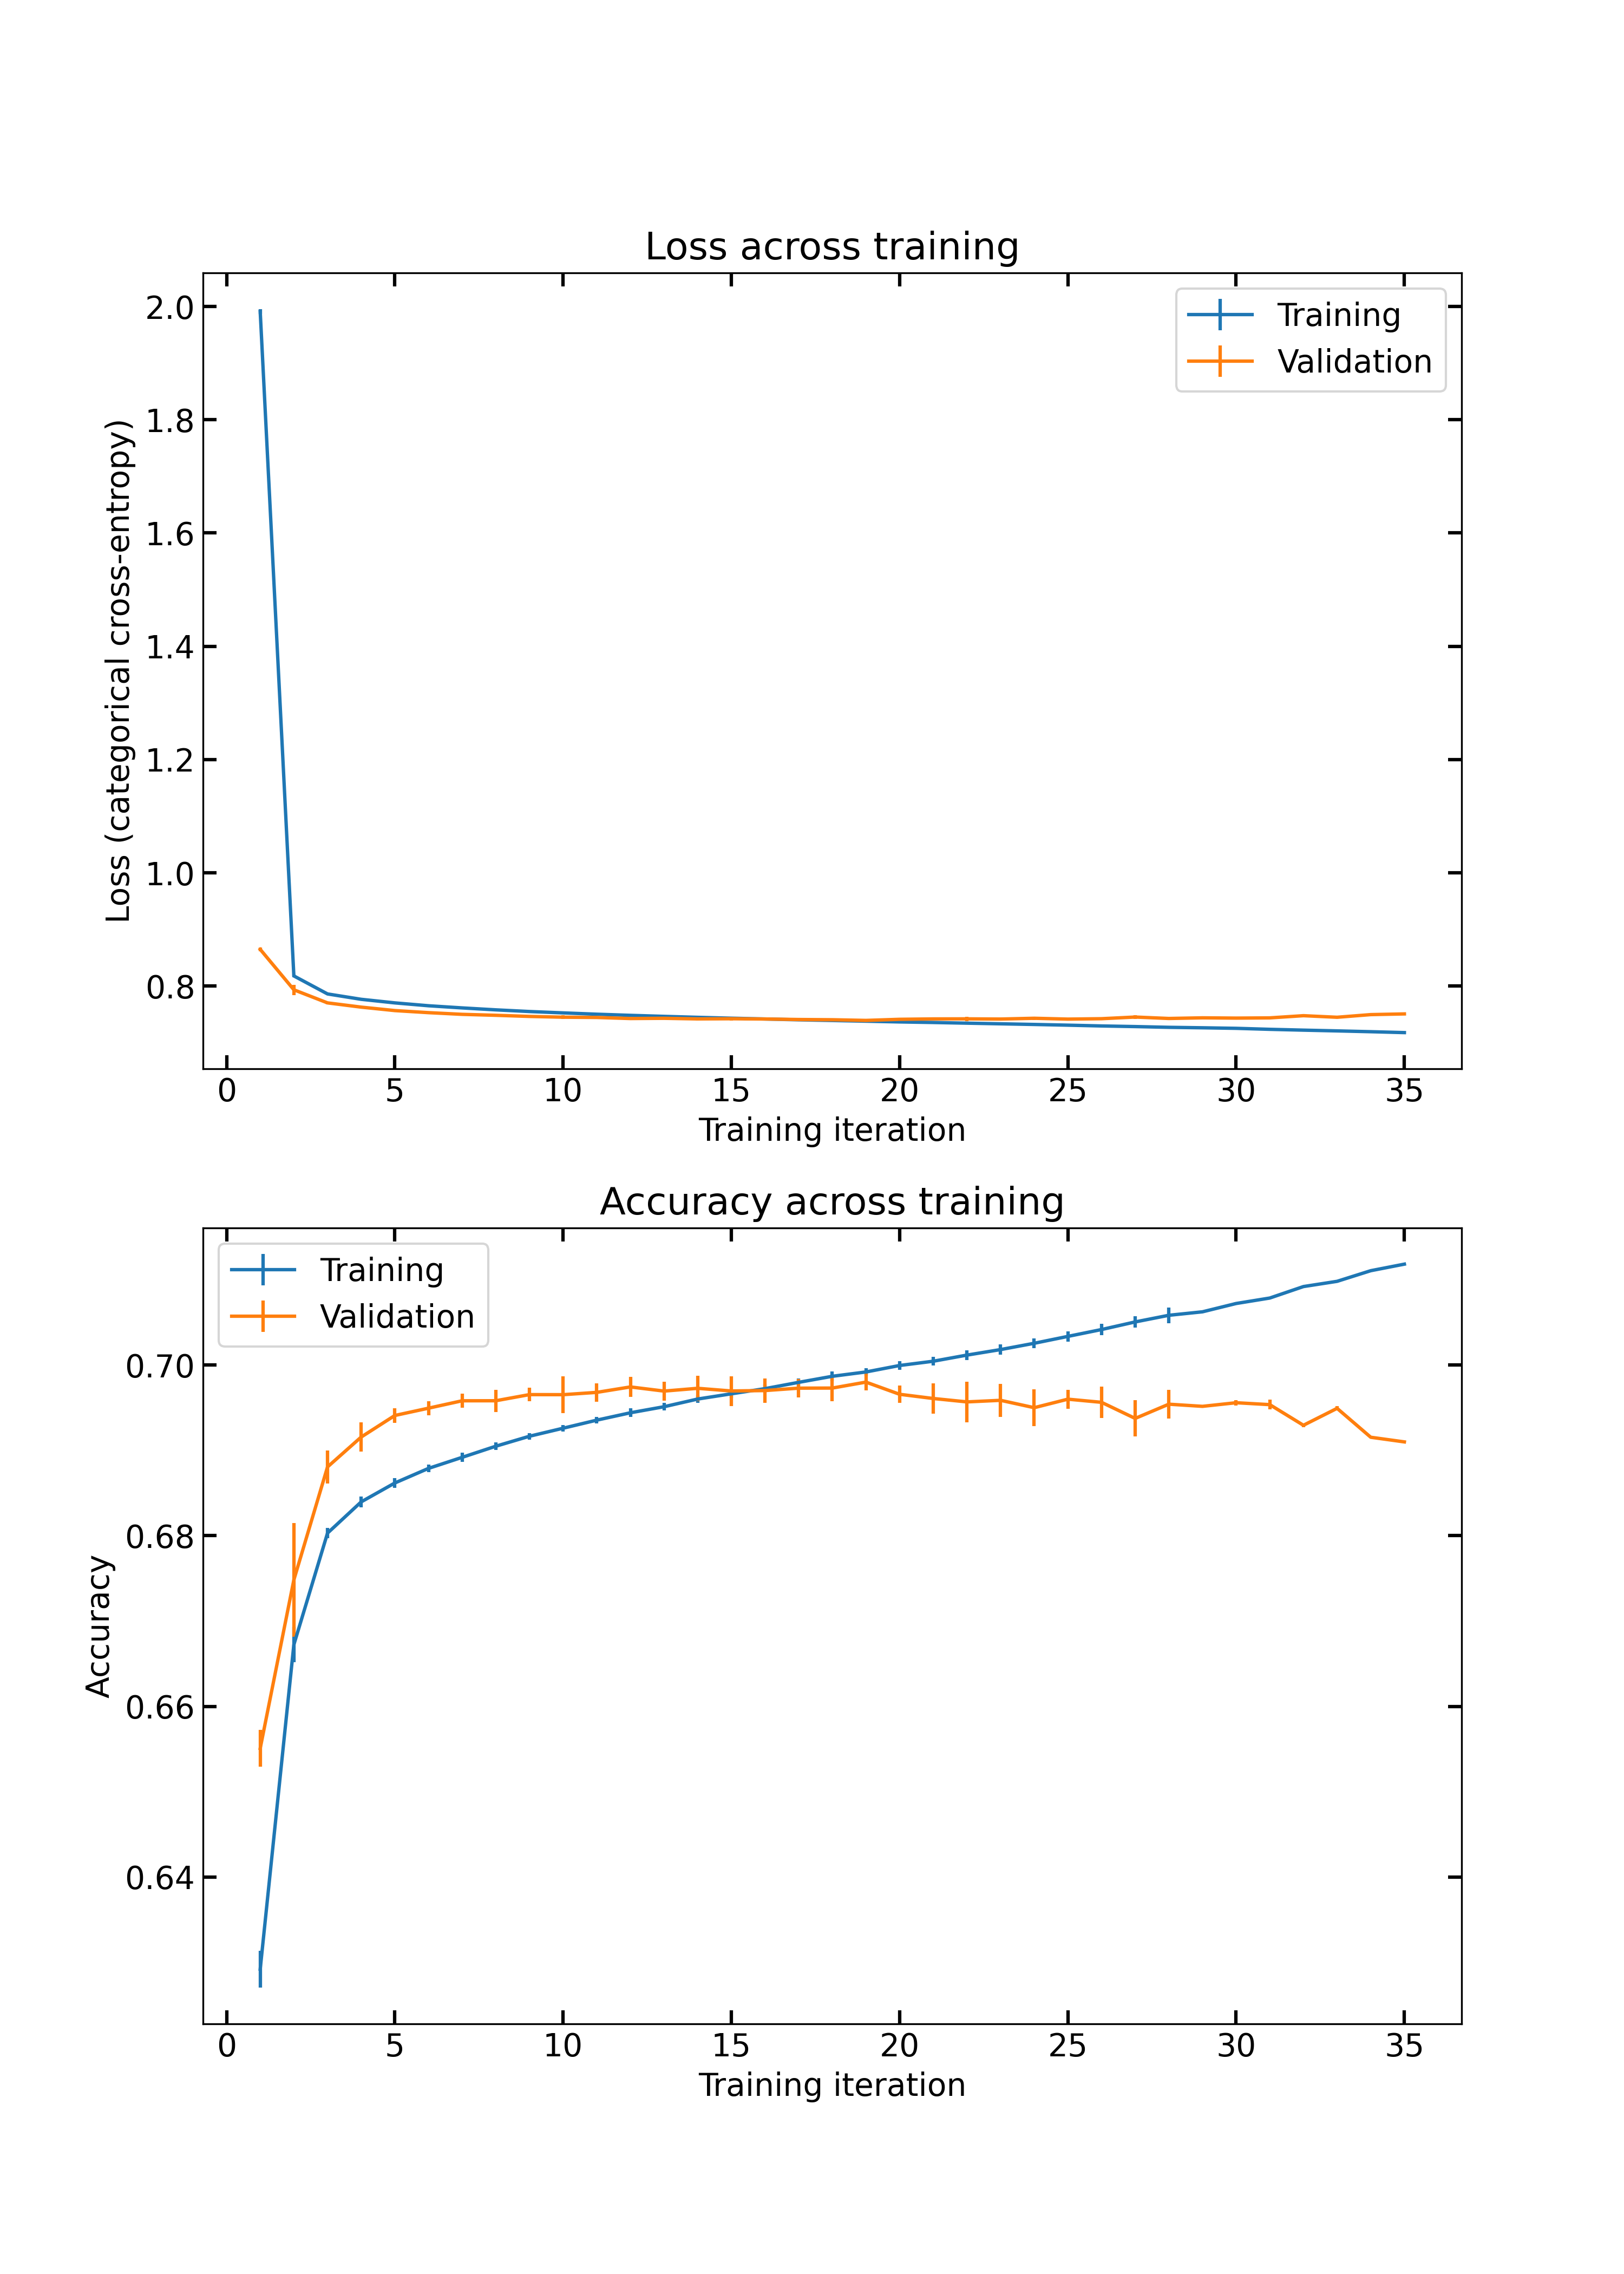
\includegraphics[width=0.95\textwidth]{loss and accuracy_CNNsq.png}
			} 
			\caption{The loss and learning curve for the CNN$^2$ model. The plotting scheme is the same as Figure~\ref{fig:CNN learning curve}.}
			\label{fig:CNNsq learning curve}
		\end{figure}
		\begin{figure}[htpb]
			\centering
			\subfloat[Ours]{
				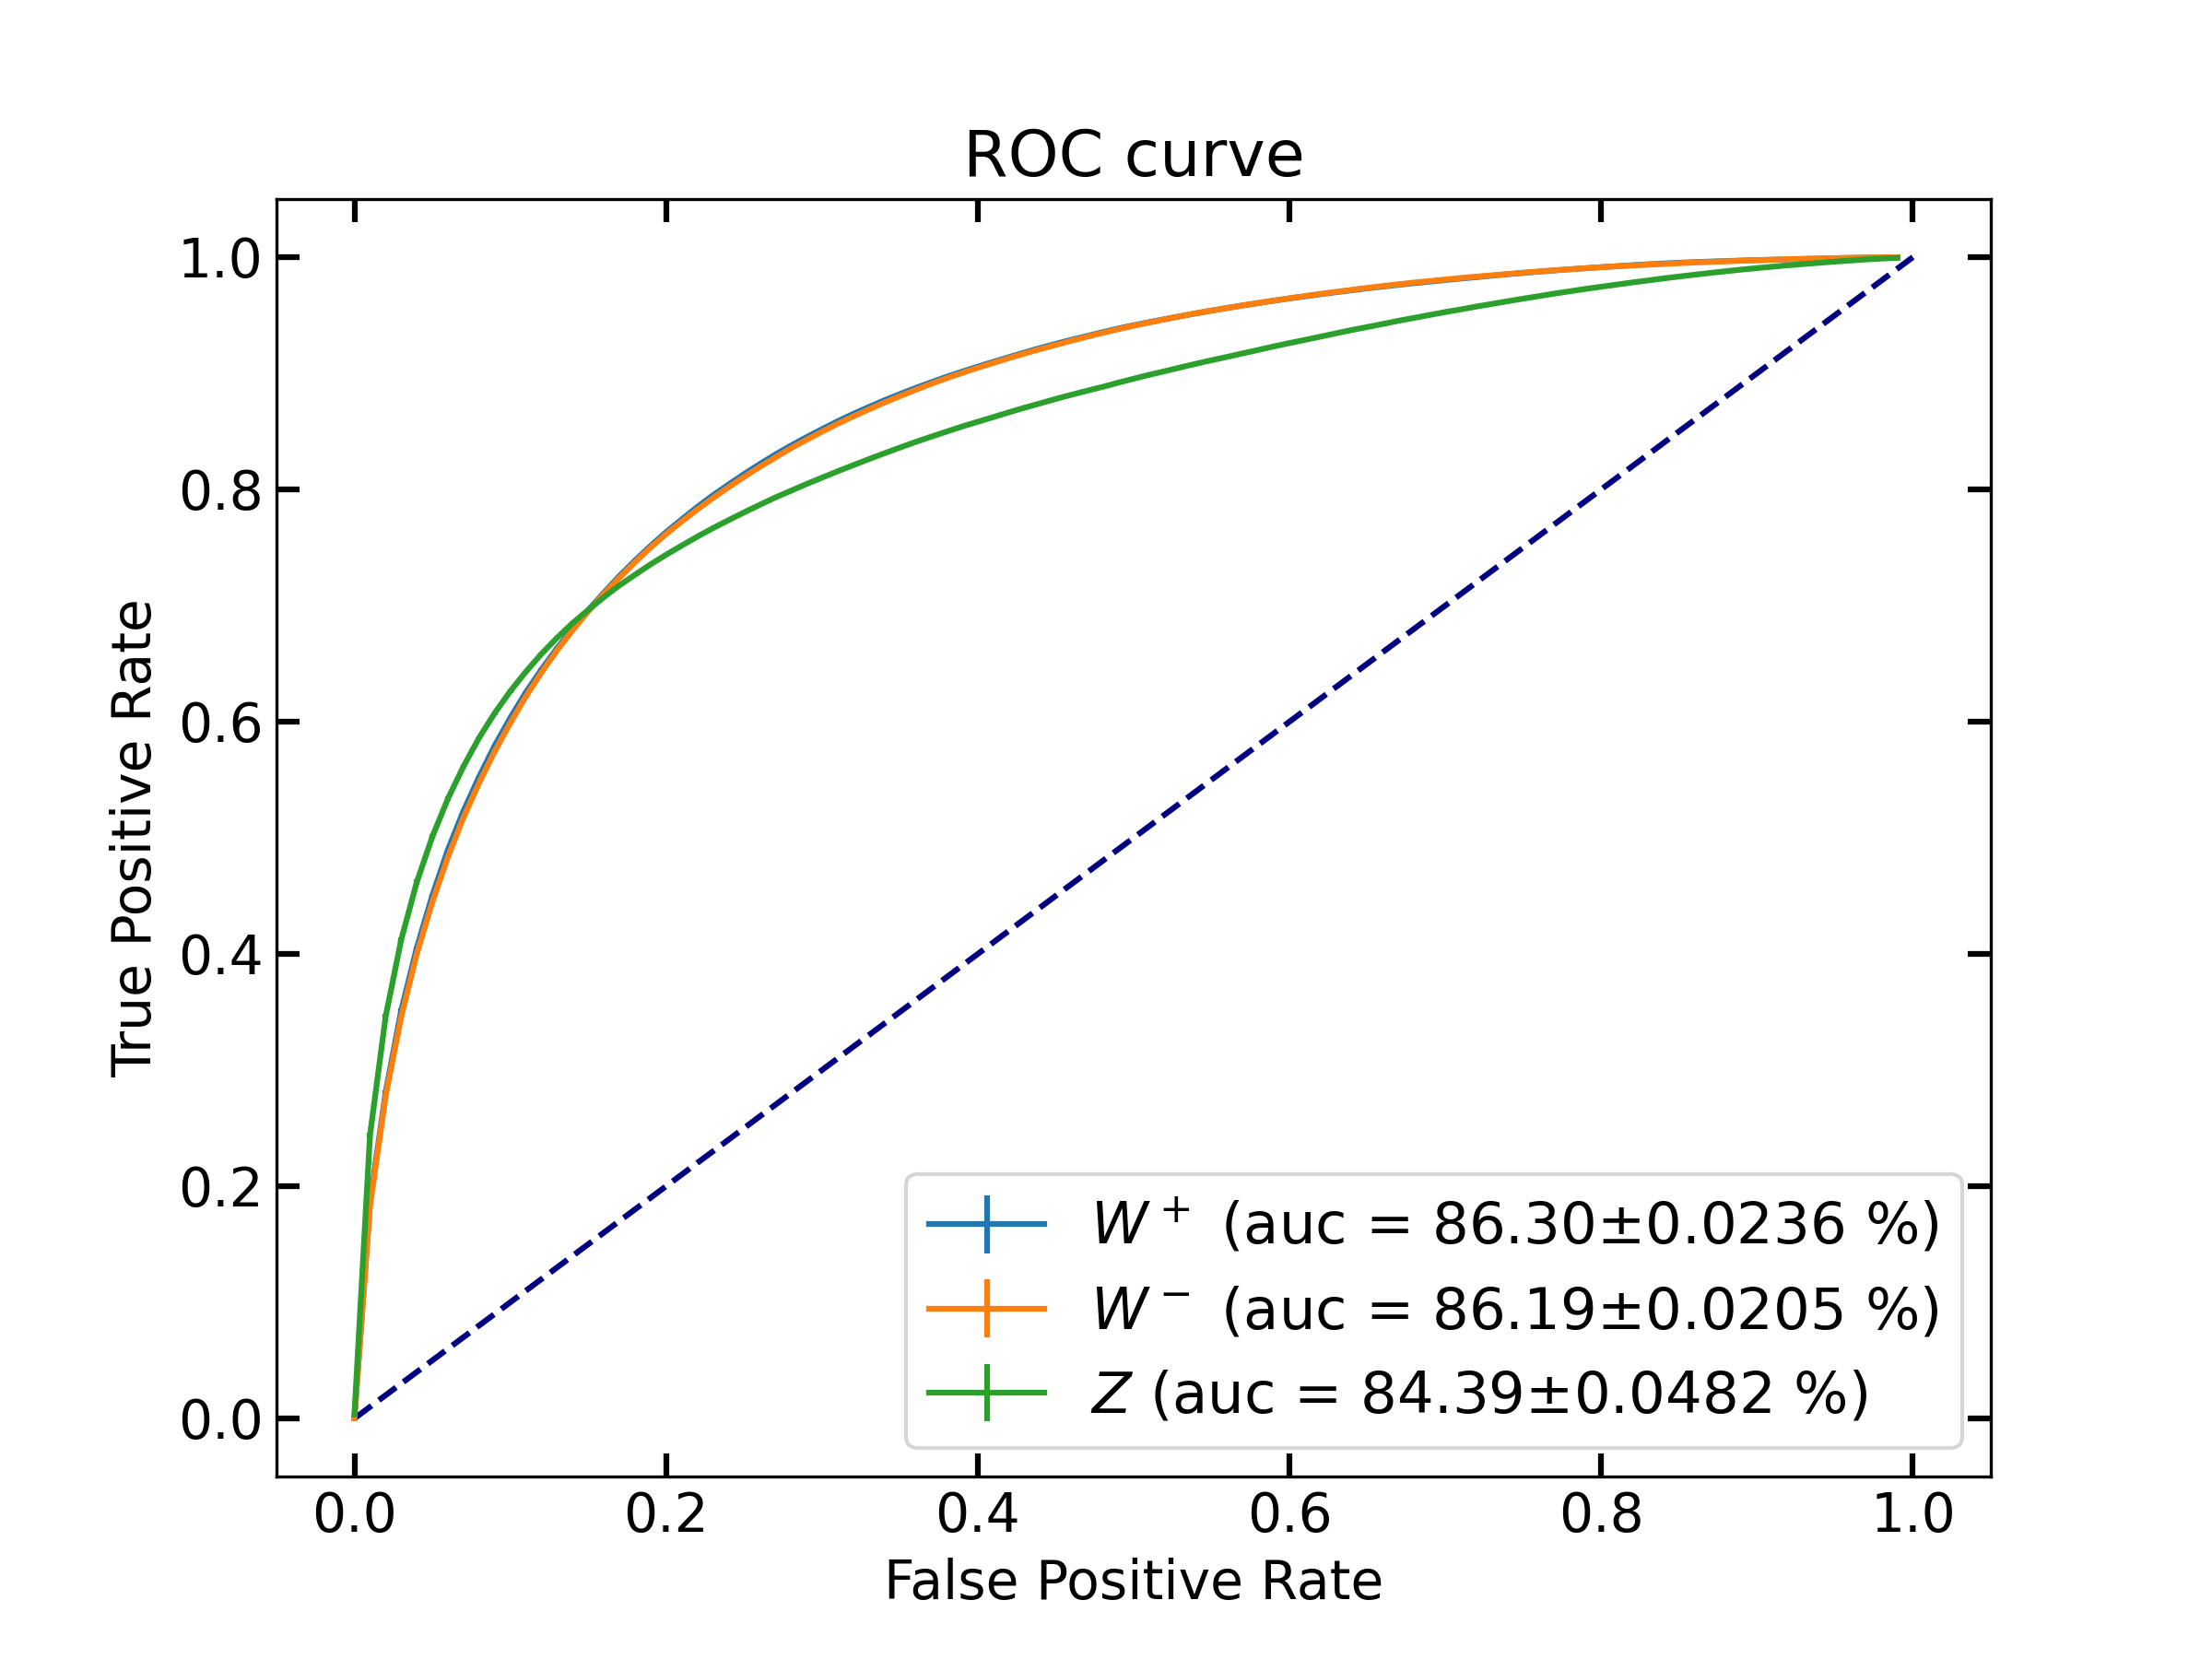
\includegraphics[width=0.95\textwidth]{roc_auc_CNNsq.png}
			} 
			\caption{The ROC curve of each vector boson for the CNN$^2$ model. The plotting scheme is the same as Figure~\ref{fig:CNN learning curve}.}
			\label{fig:CNNsq roc curve}
		\end{figure}

	% section ternary_classification (end)
\section{Correct decay width sample}% (fold)
\label{sec:correct_decay_width_sample}
	In this section, the sample is generated with the correct decay widths, i.e., the decay width of $t, W$, and $Z$ do not change and the exotic Higgses in the GM model are set to ``Auto'', meaning the decay widths are calculated by MadGraph.

	\subsection{Training results}% (fold)
	\label{sub:training_results_correct_decay_width}
		The training, validation, and testing sample size are in Table \ref{tab:sample_size_correct_decay_width}.
		\begin{table}[htpb]
			\centering
			\caption{The entries in the sum correspond to the $(W^{+}, W^{-}, Z)$ samples.}
			\label{tab:sample_size_correct_decay_width}
			\begin{tabular}{c|c|c|c}
			Case & Training set     & Validation set & Testing set   \\ \hline
			1    & $223k+232k+202k$ & $56k+57k+50k$ & $69k+72k+62k$\\
			\end{tabular}
		\end{table}

		The training results are summarized in Table \ref{tab:training_result_correct_decay_width}.
		\begin{table}[htpb]
			\centering
			\caption{The training results of correct decay width sample. The training results of CNN and CNN$^2$ are presented with an average and a standard deviation. These values are derived from 10 times training with the same dataset. Yet, the ACC value of each boson is only derived from a single result.}
			\label{tab:training_result_correct_decay_width}
			\resizebox{\textwidth}{!}{
			\begin{tabular}{c|c|c|cc|cc|cc}
										&					  &             & \multicolumn{2}{c|}{$W^{+}$} & \multicolumn{2}{c|}{$W^{-}$} & \multicolumn{2}{c}{$Z$} \\
										& Sample			  & Overall ACC & AUC        & ACC       & AUC        & ACC       & AUC       & ACC       \\ \hline
				BDT $\kappa=0.30$       &\multirow{3}{*}{1}    & 65.1 & 82.6 & 77.5 & 82.5 & 77.0 & 79.2 & 77.4\\
				CNN $\kappa=0.15$       &					   & 68.24$\pm$0.04 & 85.72$\pm$0.02 & (79.5) & 85.58$\pm$0.02 & (79.1) & 81.64$\pm$0.05 & (79.8)\\
				CNN$^2$ $\kappa=0.15$   &					   & 68.26$\pm$0.13 & 85.55$\pm$0.04 & (79.5) & 85.41$\pm$0.05 & (79.0) & 82.22$\pm$0.08 & (80.2)\\
			\end{tabular}
			}
		\end{table}
		The results are worse than Sec.\ref{sec:ternary_classification}. It seems that the decay width of $t, W$, and  $Z$ will affect the training results.

		Figure \ref{fig:CNN learning curve_correct_decay_width} is CNN's loss and accuracy curve. Figure \ref{fig:CNN roc curve_correct_decay_width} is CNN's ROC curve.
		\begin{figure}[htpb]
			\centering
			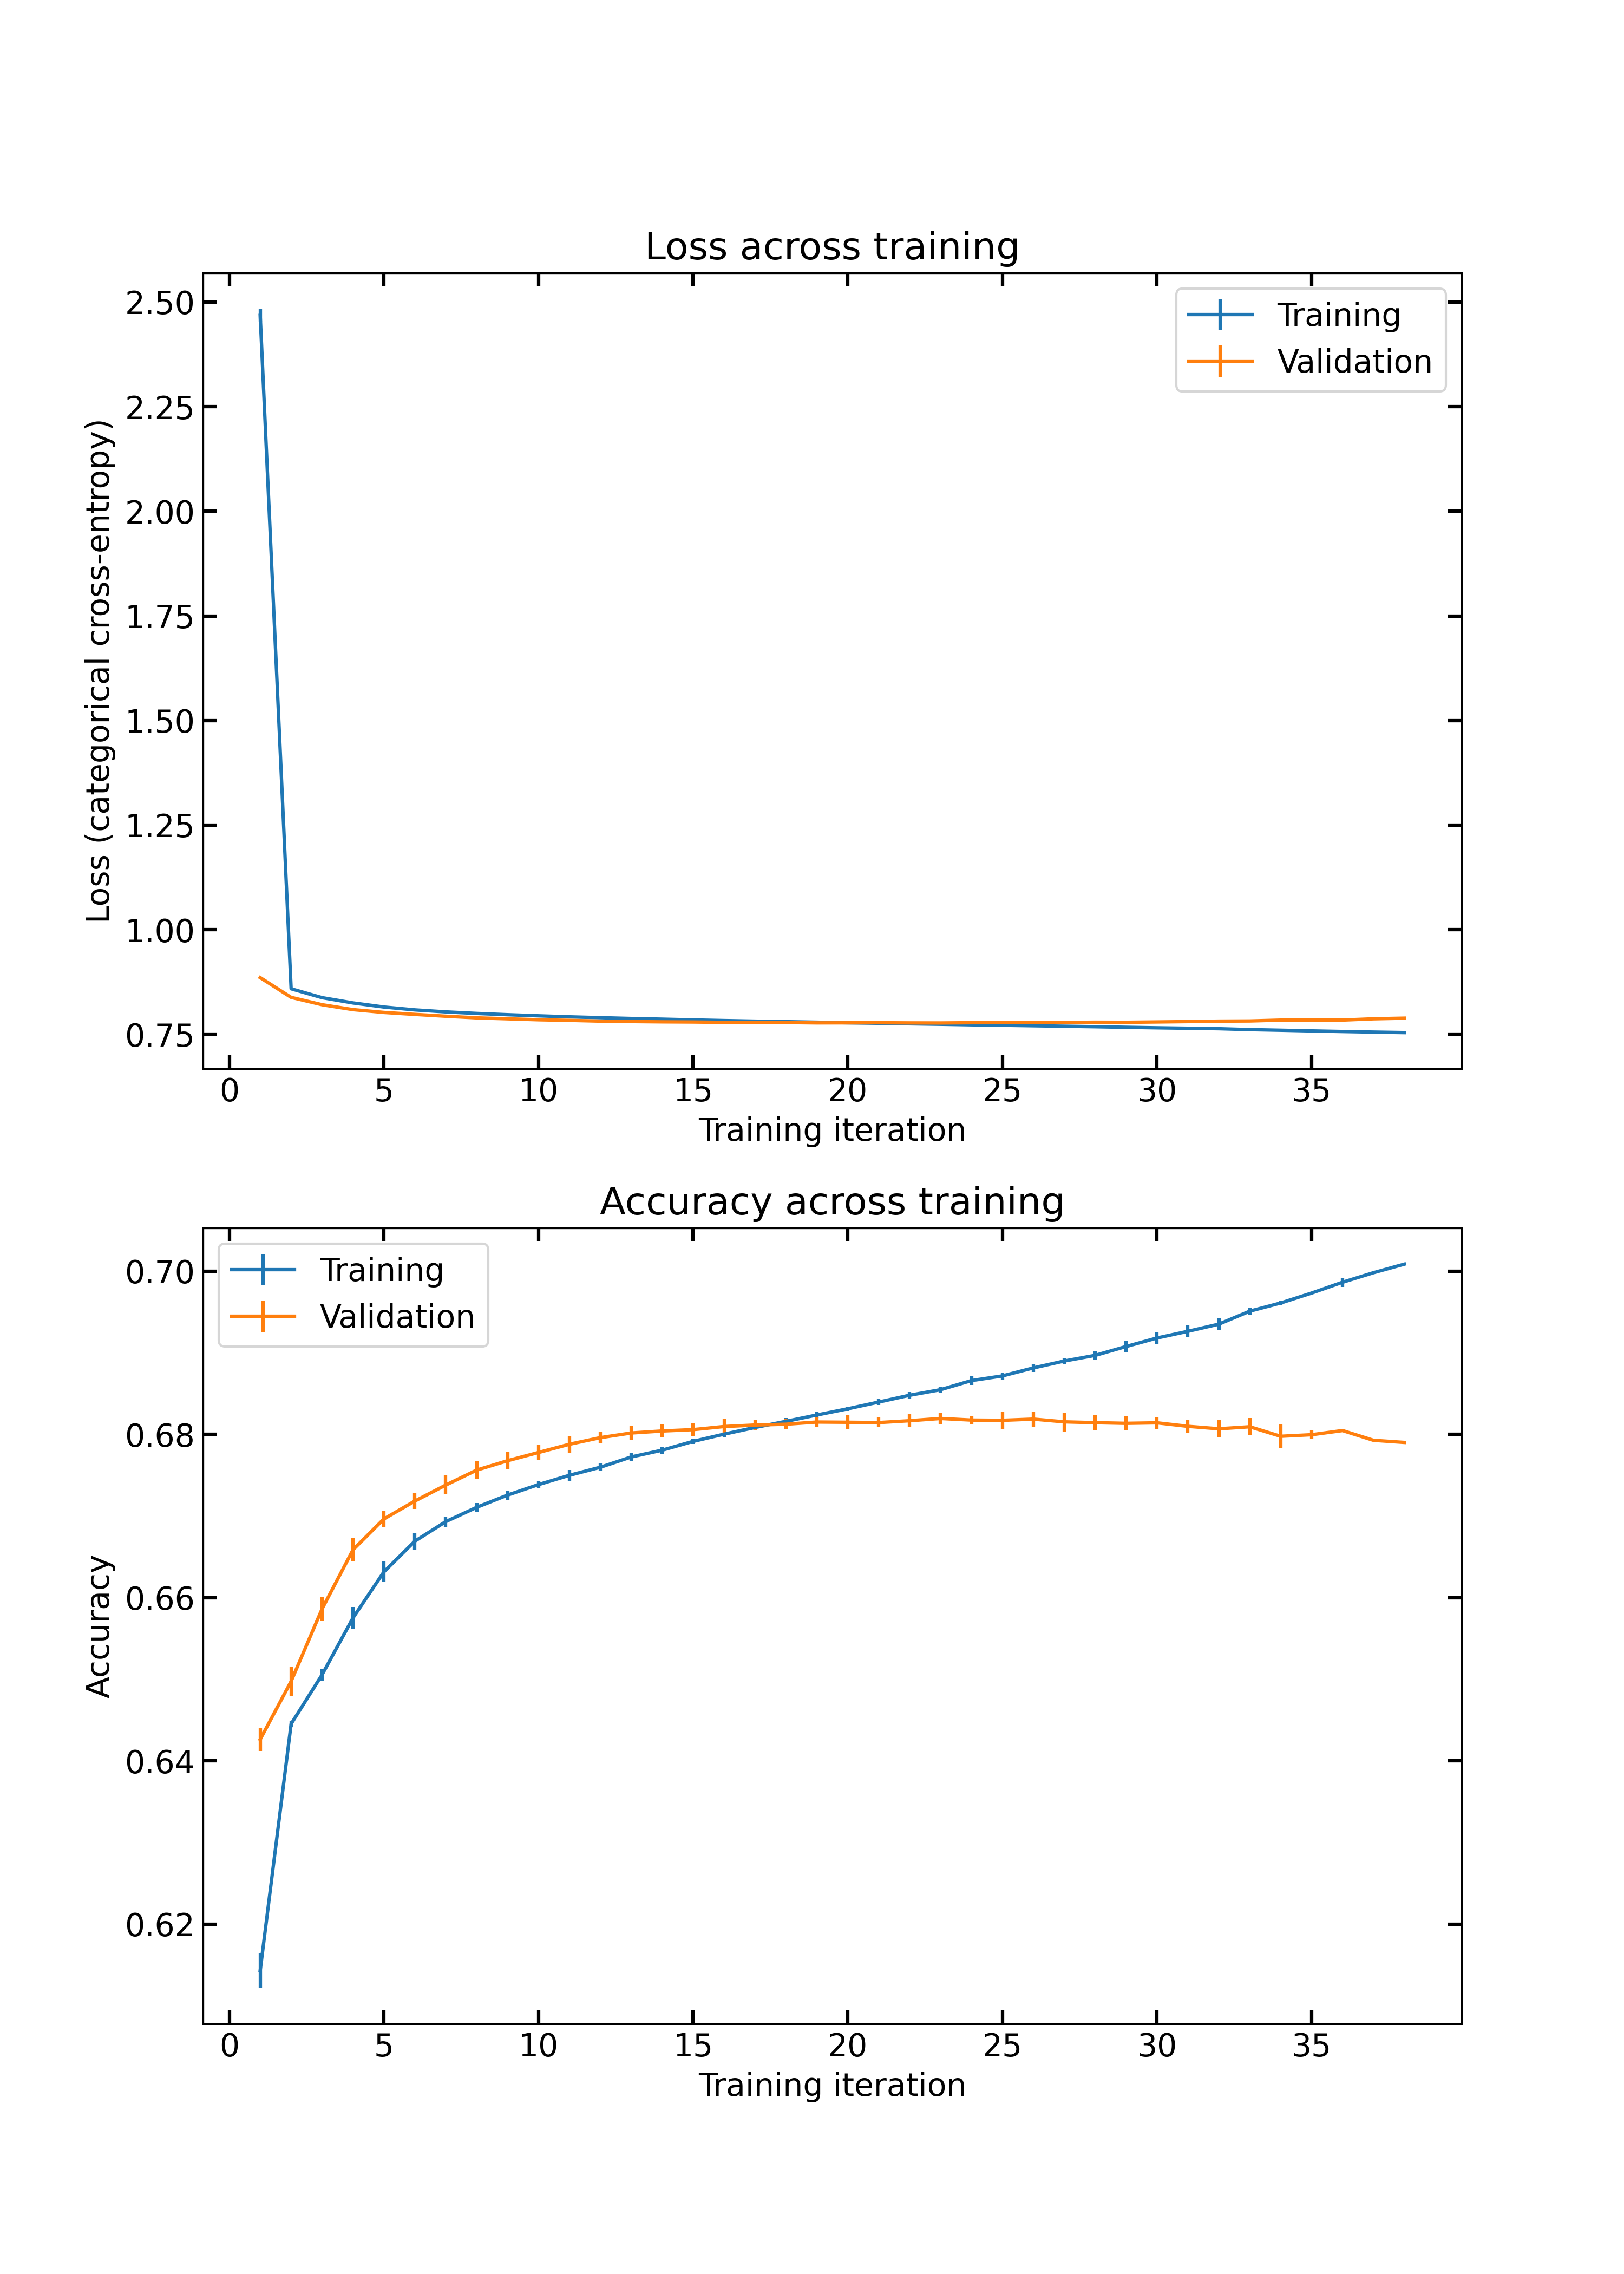
\includegraphics[width=0.90\textwidth]{CNN_loss_and_accuracy_correct_width.png}
			\caption{The loss and accuracy curve for the CNN model. Both of them are demonstrated with the average value (solid curve) and the first standard deviation range (error bar).}
			\label{fig:CNN learning curve_correct_decay_width}
		\end{figure}
		\begin{figure}[htpb]
			\centering
			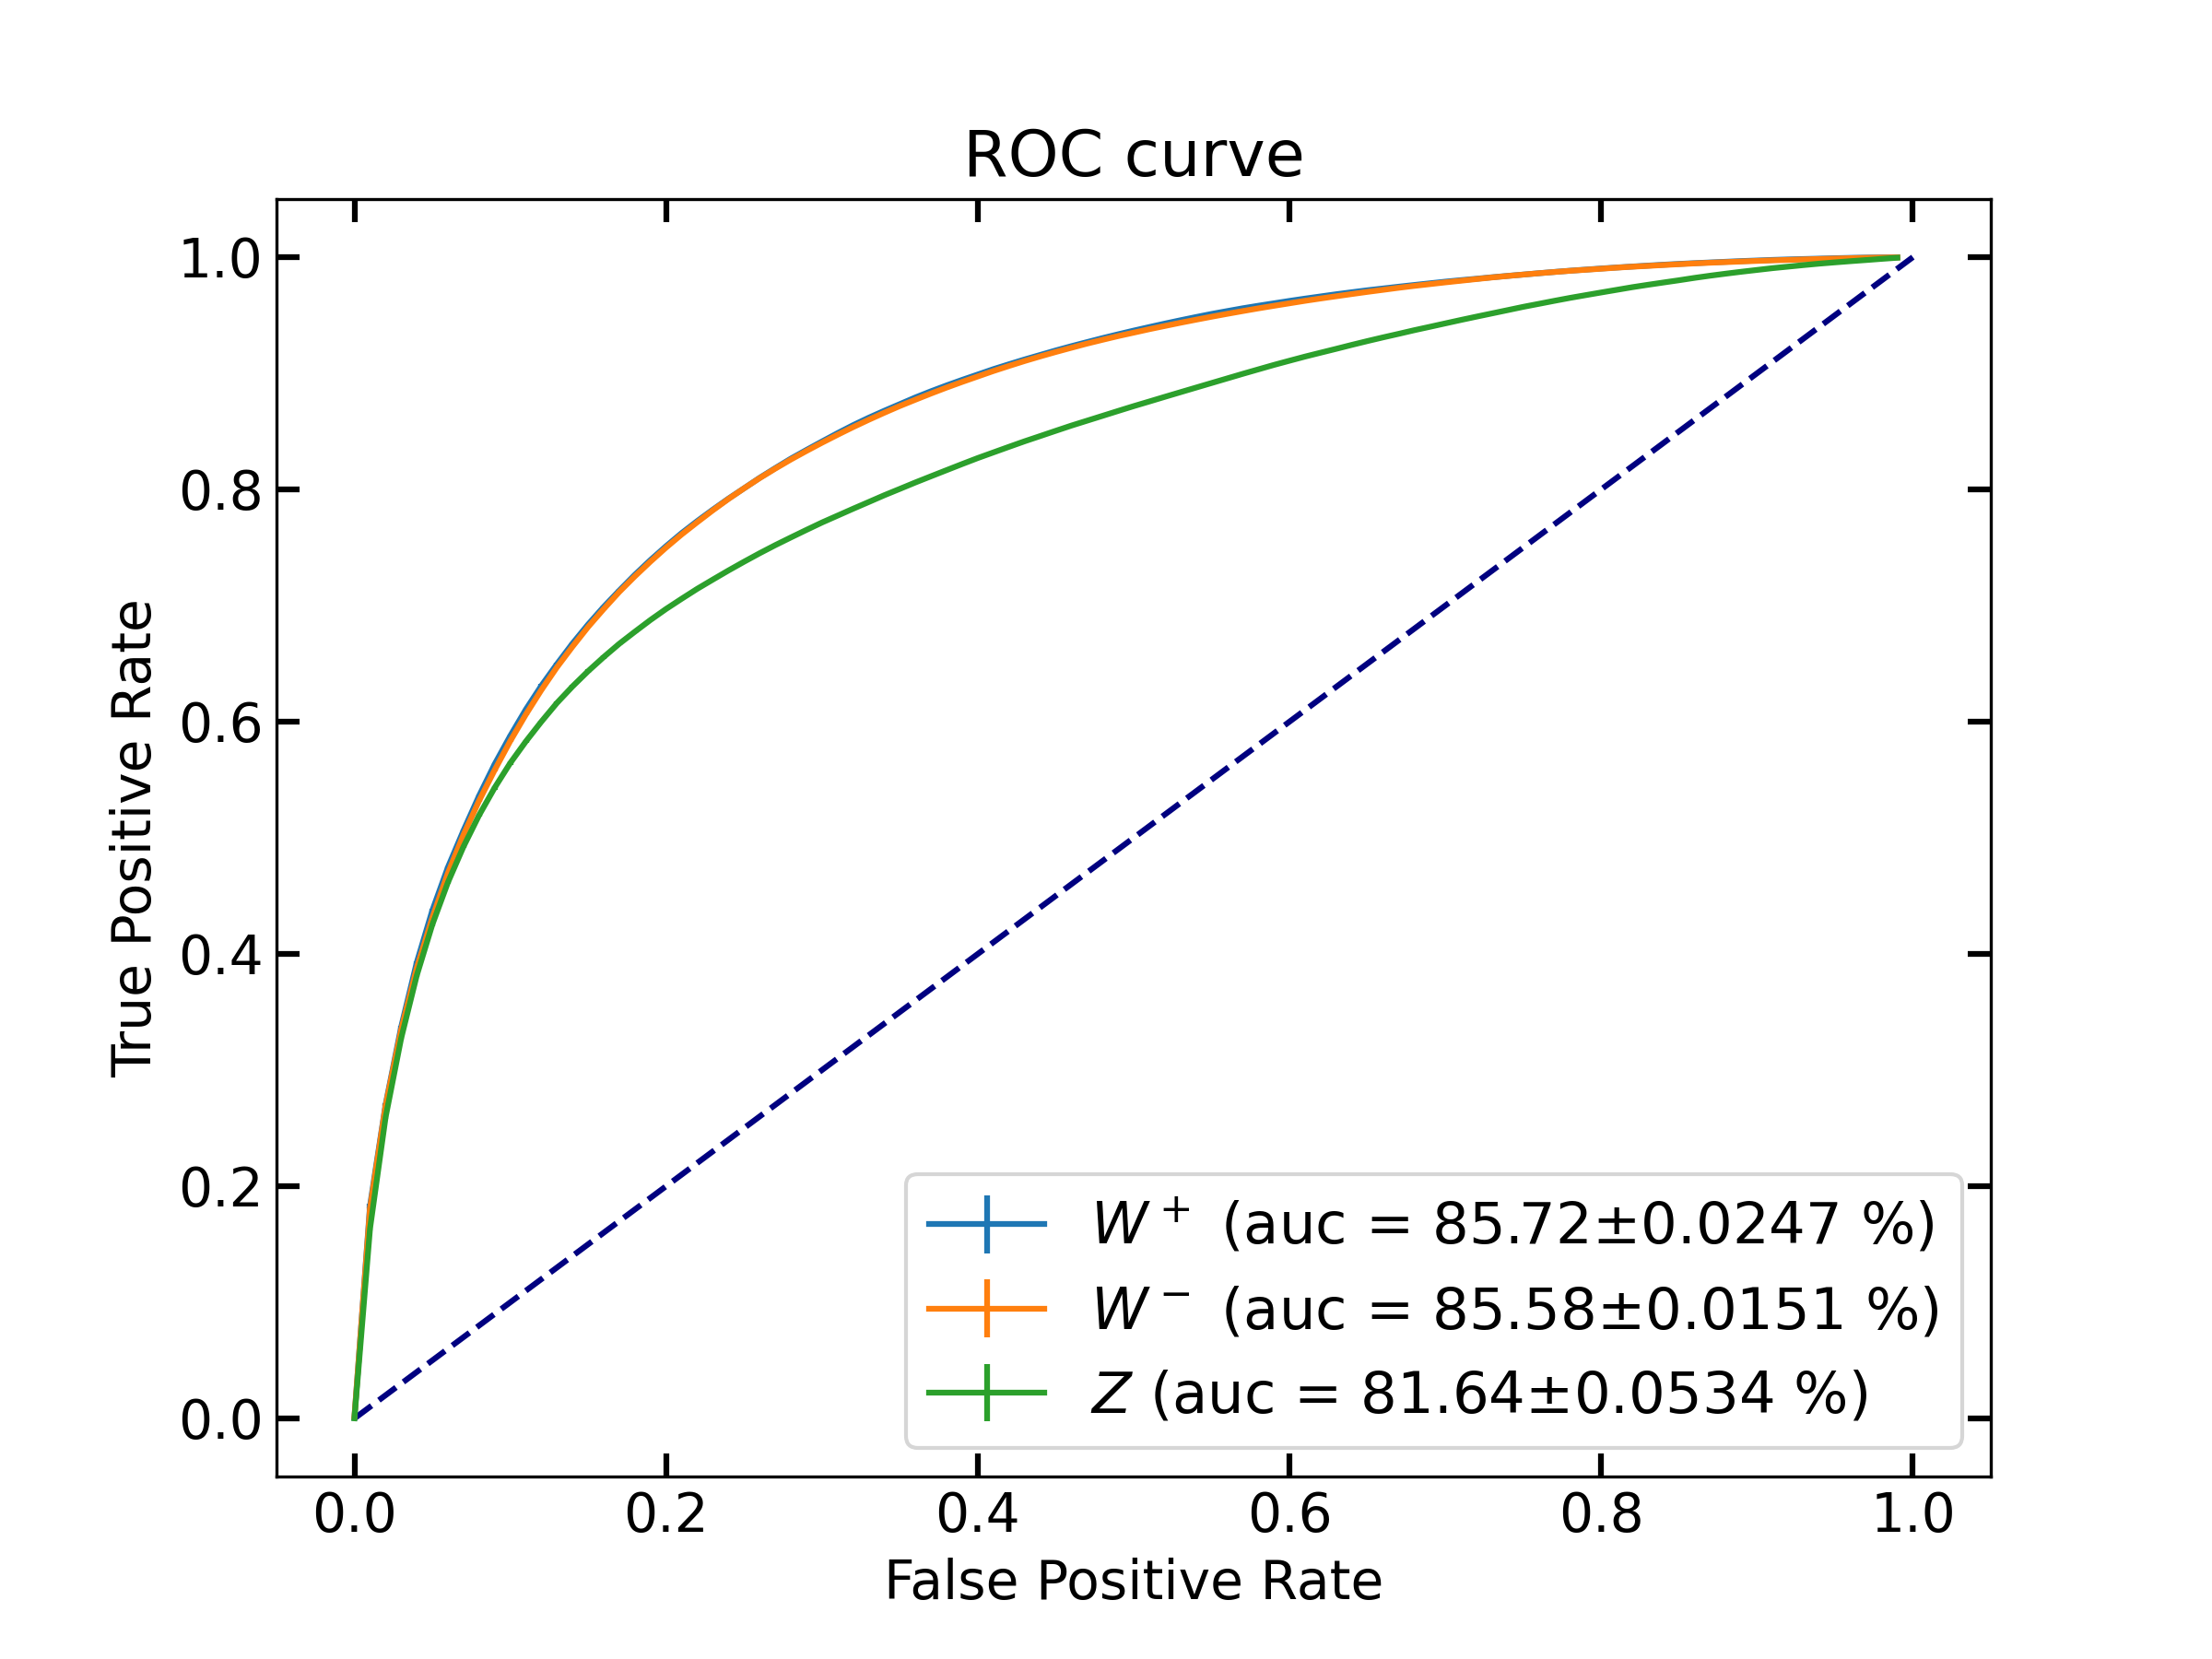
\includegraphics[width=0.95\textwidth]{CNN_roc_auc_correct_width.png}
			\caption{The ROC curve of each vector boson for the CNN model. The plotting scheme is the same as Figure \ref{fig:CNN learning curve_correct_decay_width}.}
			\label{fig:CNN roc curve_correct_decay_width}
		\end{figure}
		
		Figure \ref{fig:CNNsq learning curve_correct_decay_width} is CNN${}^2$'s loss and accuracy curve. Figure \ref{fig:CNNsq roc curve_correct_decay_width} is CNN${}^2$'s ROC curve.
		\begin{figure}[htpb]
			\centering
			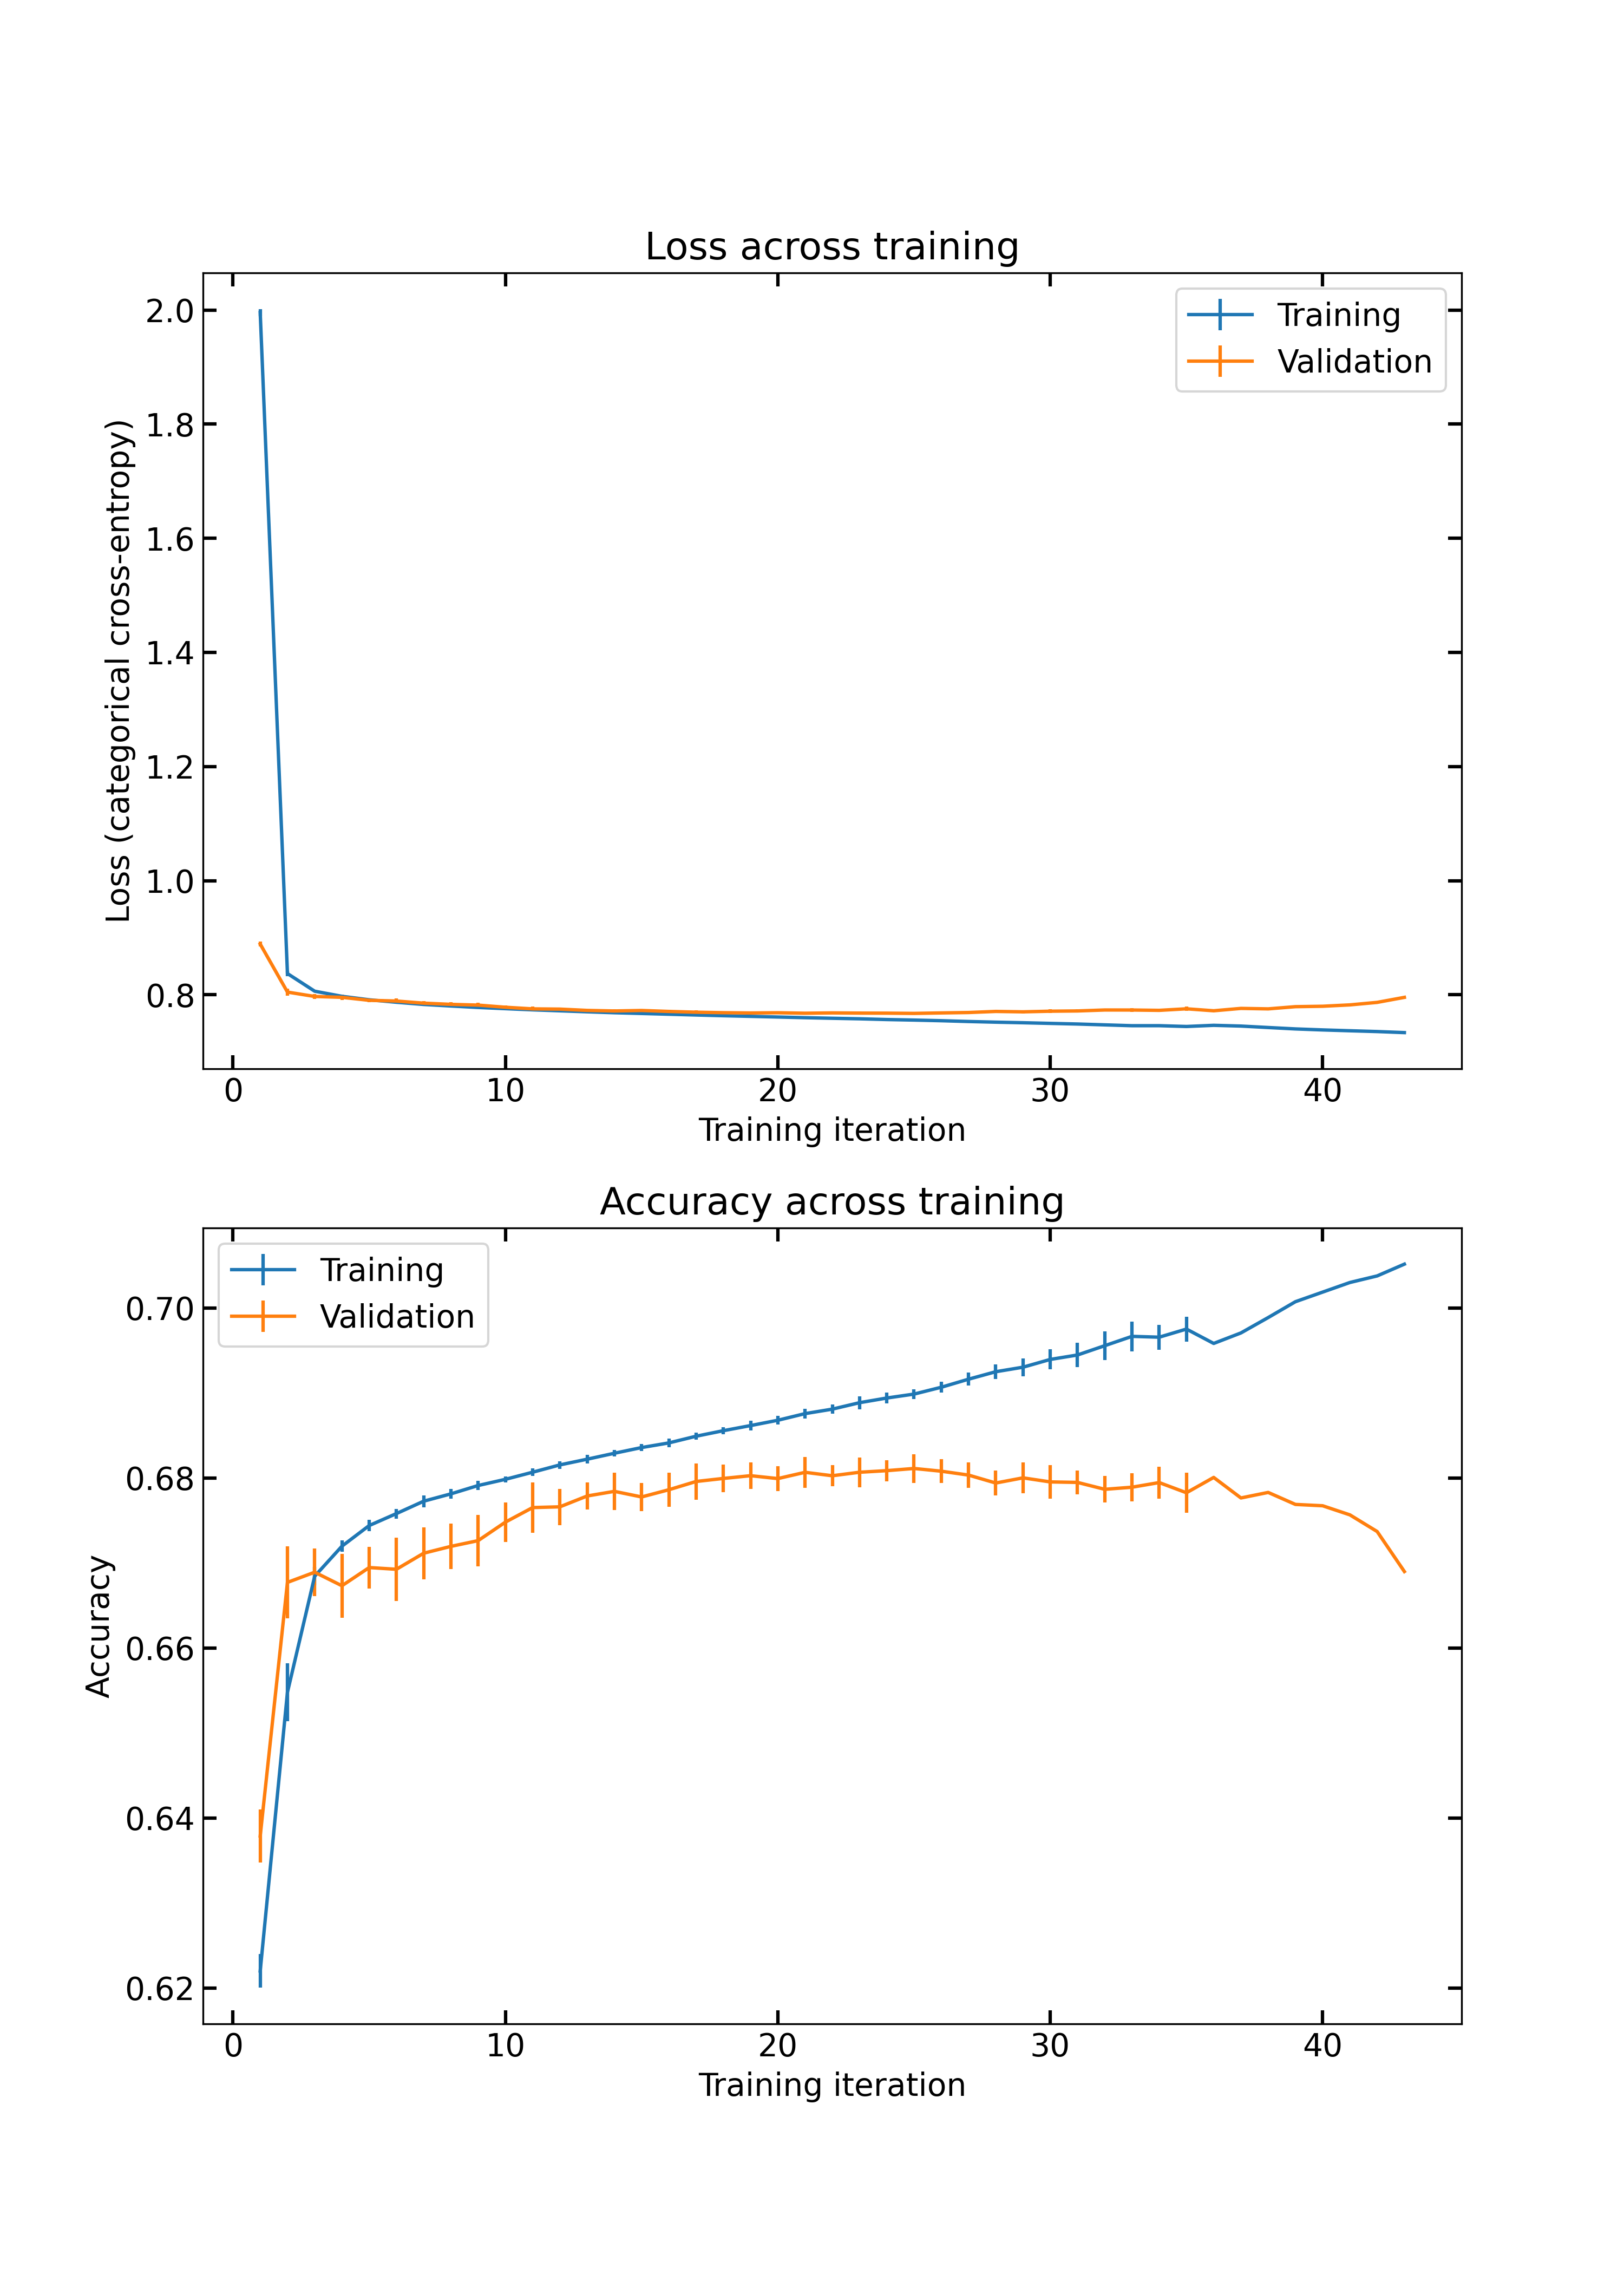
\includegraphics[width=0.90\textwidth]{CNNsq_loss_and_accuracy_correct_width.png}
			\caption{The loss and accuracy curve for the CNN$^2$ model. The plotting scheme is the same as Figure \ref{fig:CNN learning curve_correct_decay_width}.}
			\label{fig:CNNsq learning curve_correct_decay_width}
		\end{figure}
		\begin{figure}[htpb]
			\centering
			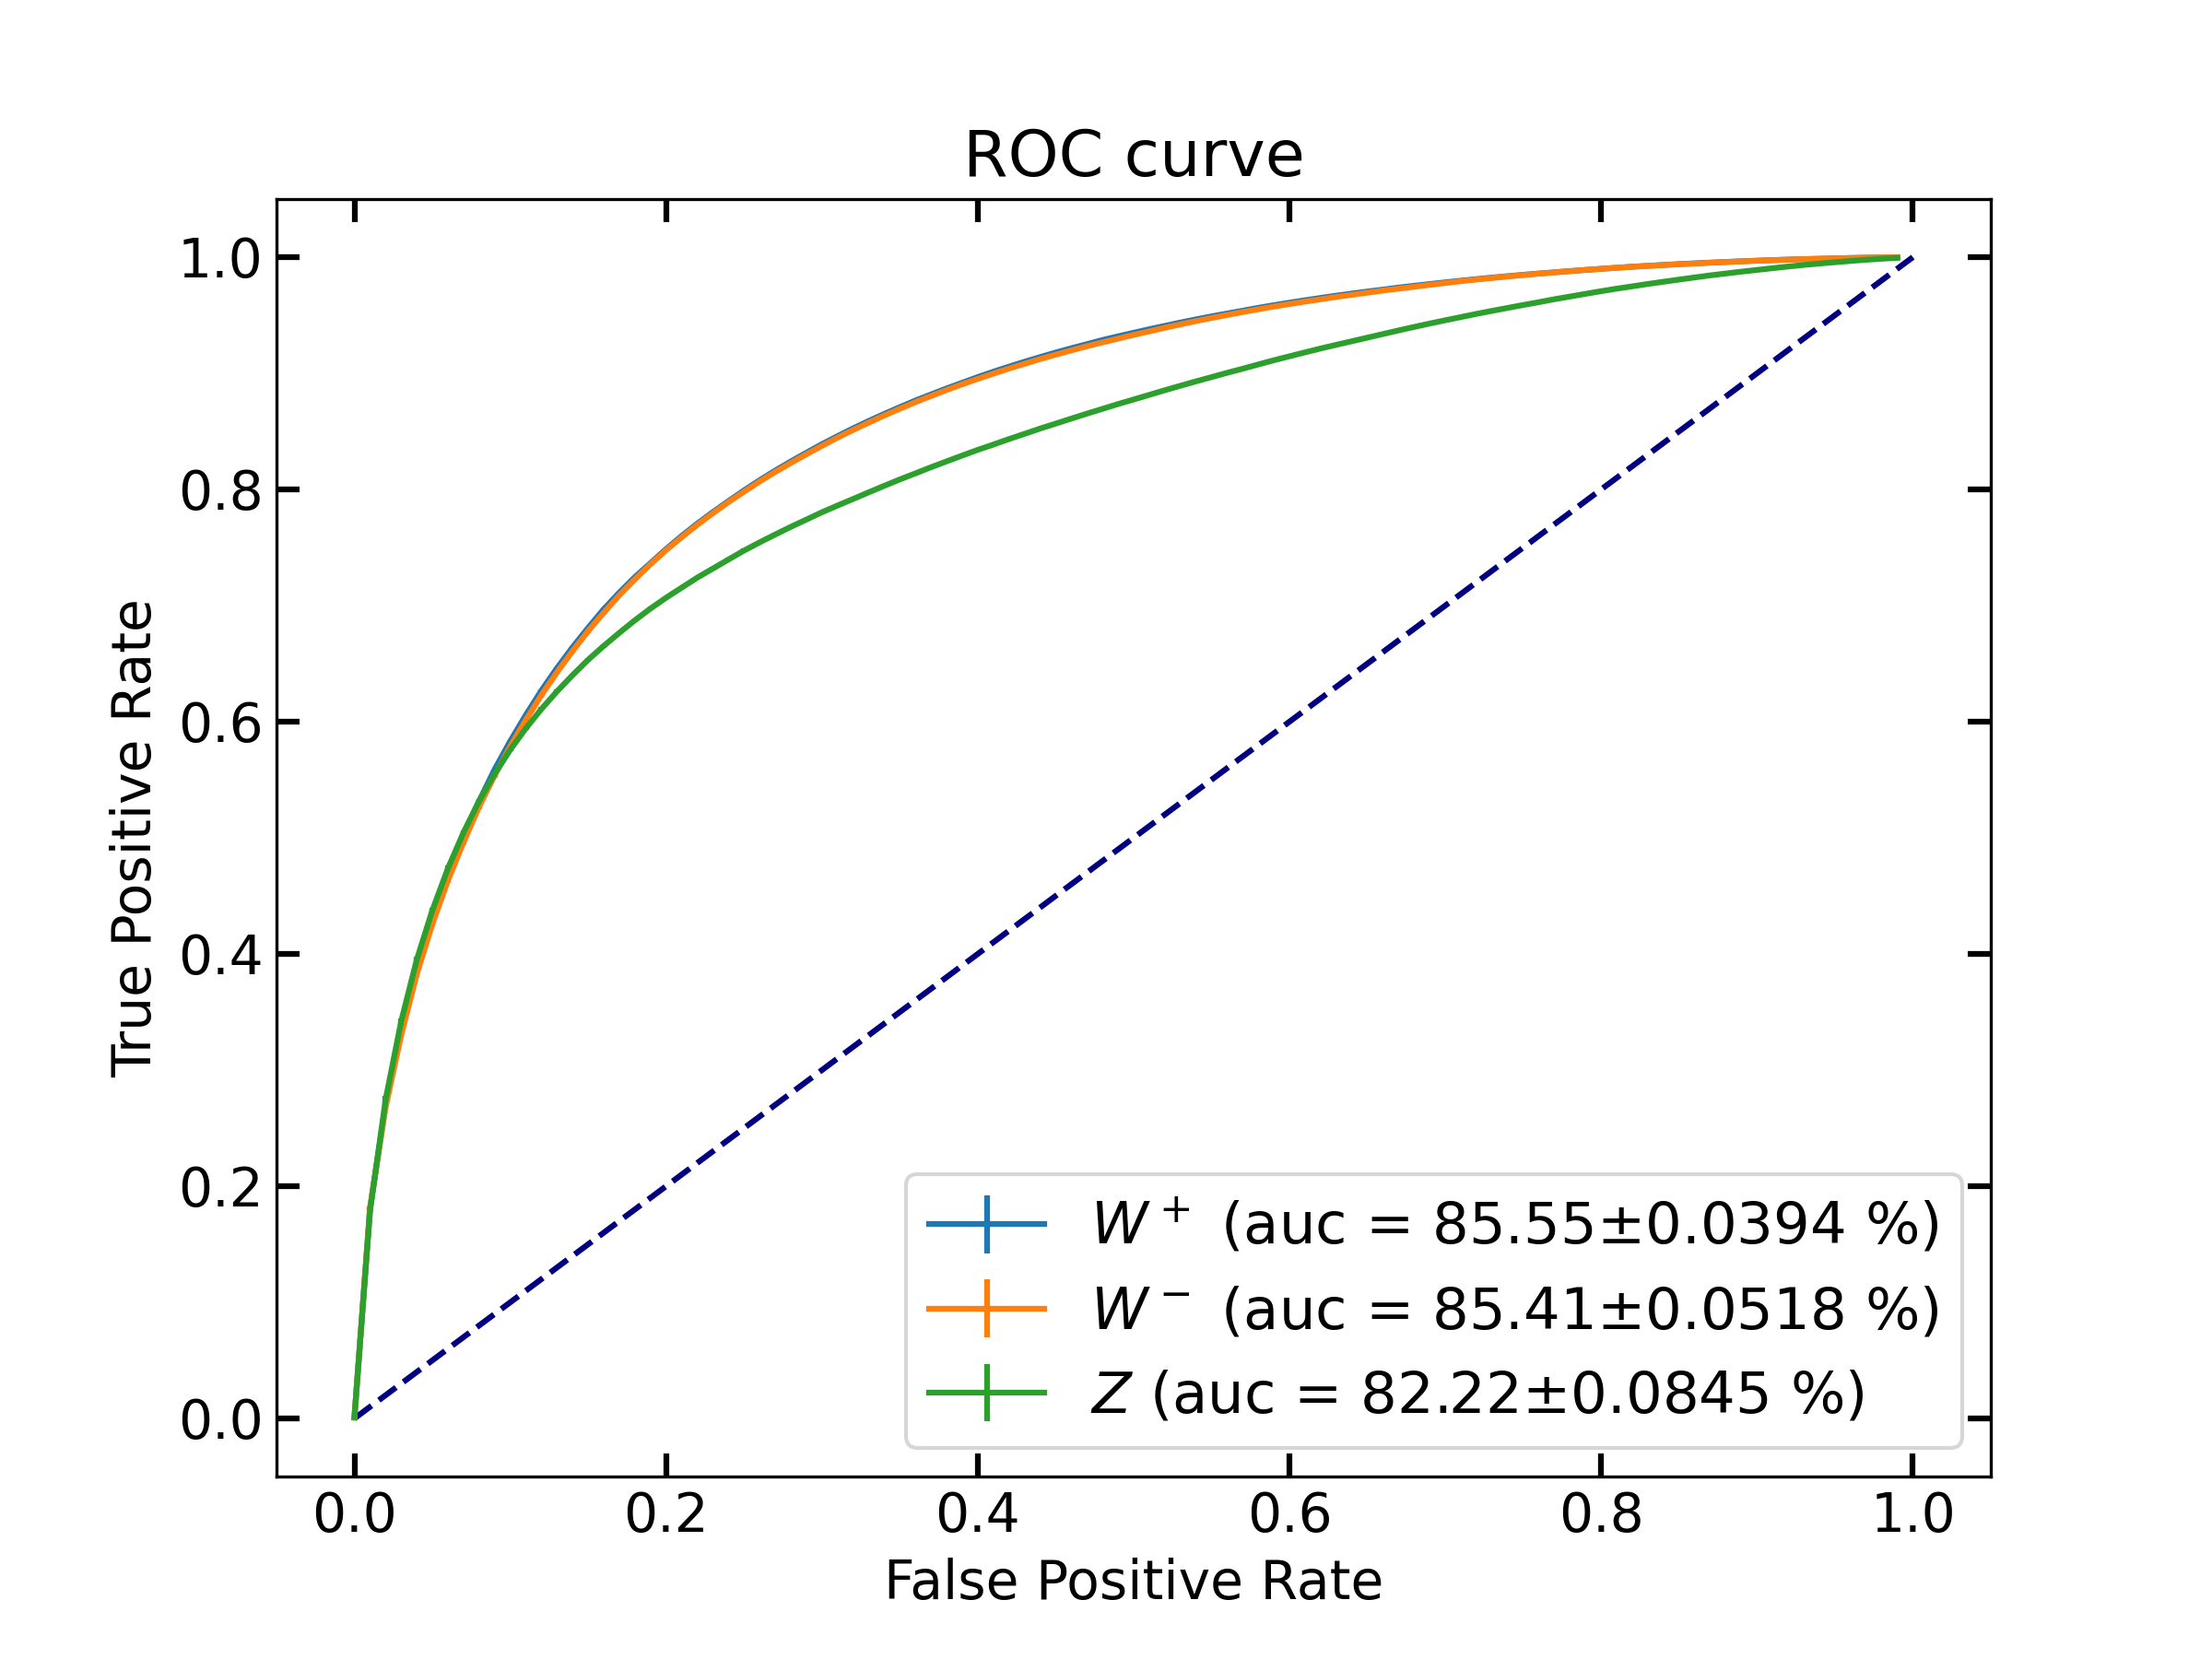
\includegraphics[width=0.95\textwidth]{CNNsq_roc_auc_correct_width.png}
			\caption{The ROC curve of each vector boson for the CNN$^2$ model. The plotting scheme is the same as Figure \ref{fig:CNN learning curve_correct_decay_width}.}
			\label{fig:CNNsq roc curve_correct_decay_width}
		\end{figure}

	% subsection training_results (end)
% section correct_decay_width_sample (end)		

\end{document} 
